\section{Appendix}

\subsection{Figures for calculation of $E_g$}
\label{sec:appendix_band_gap_plots}
\begin{figure}[htpb]
    \centering
    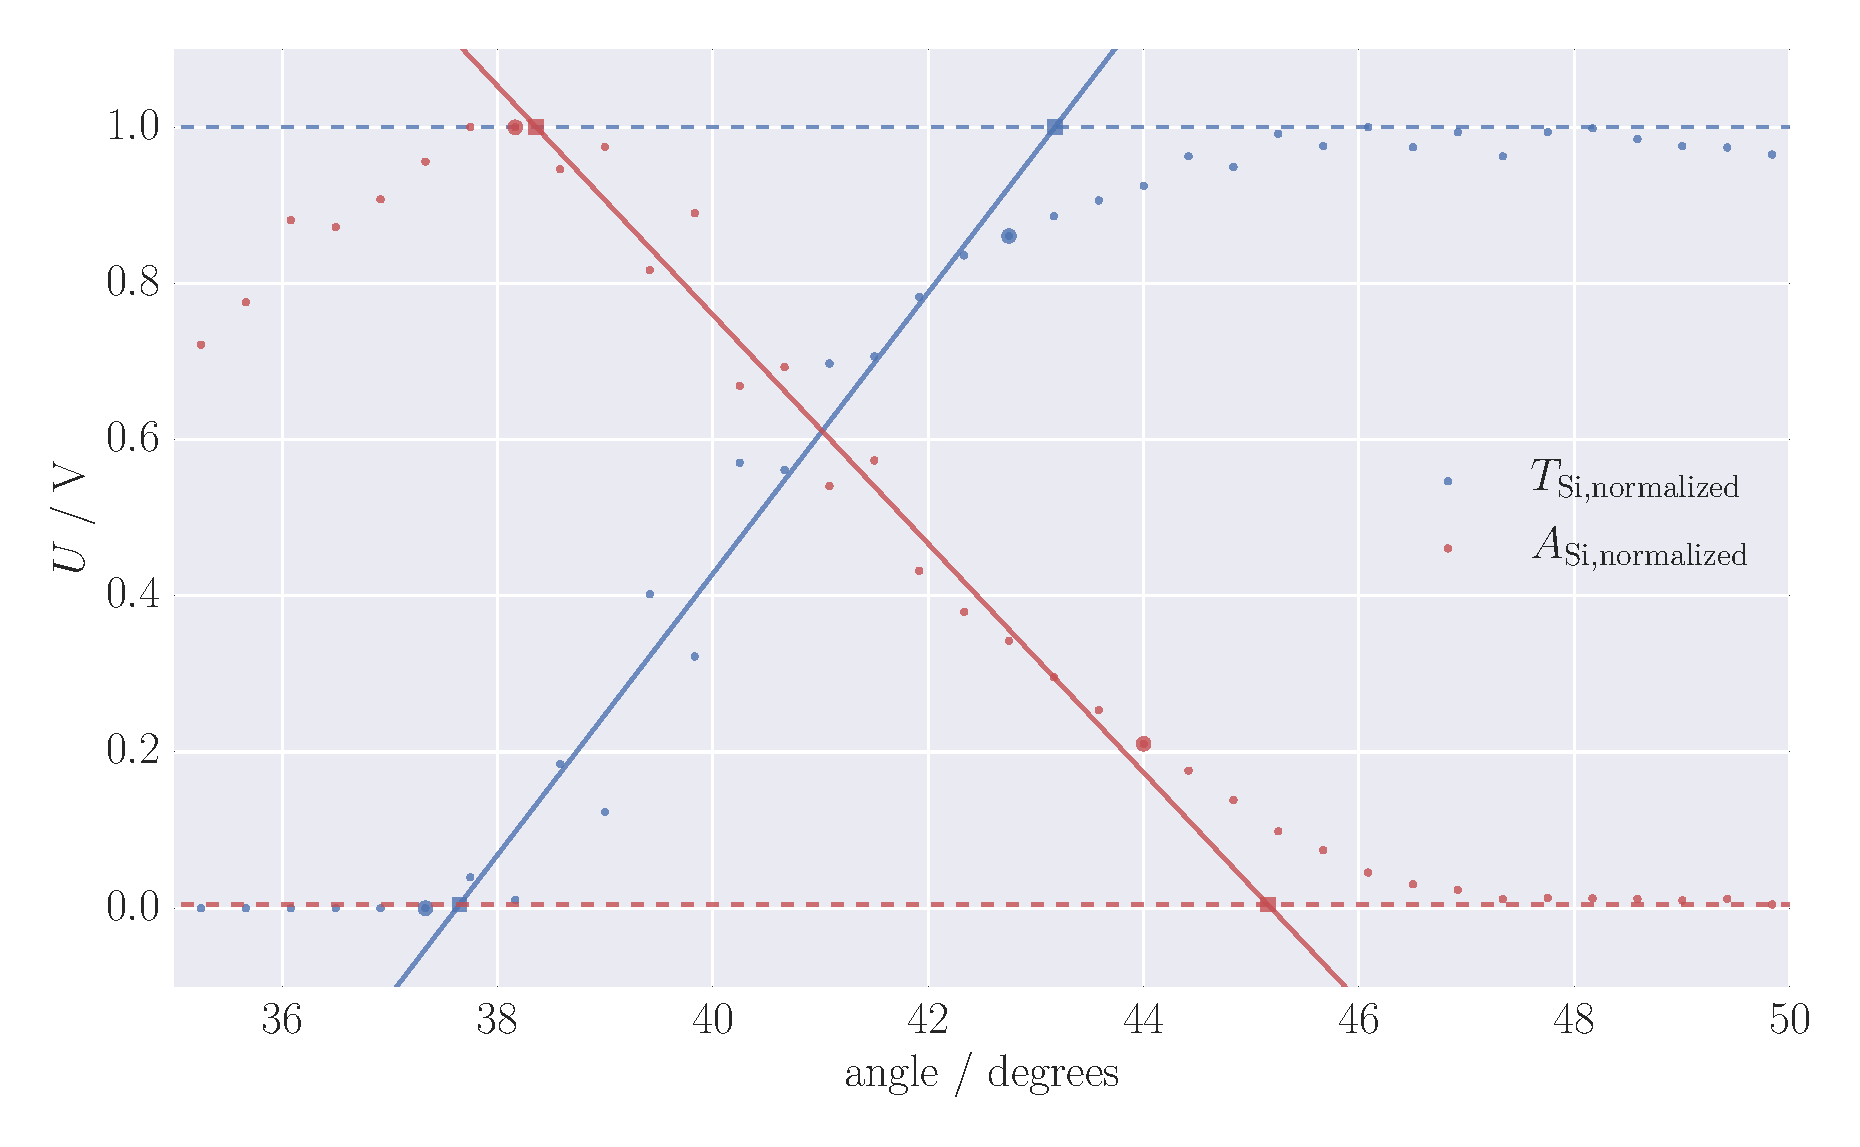
\includegraphics[width=1.0\linewidth]{figures/band_gap_result_Si_right}
    \caption{
        Result of the procedure fitting straight lines through the points 
        at the transition from transmitting to absorbing characteristic
        for the peaks on the right side ($\alpha > 0$) with the Si sample.
        For indications on the symbols, refer to figure 
        \ref{fig:band_gap_result_Si_left}. 
        }
    \label{fig:band_gap_result_Si_right}
\end{figure}
\begin{figure}
    \centering
    \begin{subfigure}[b]{\pltw}
        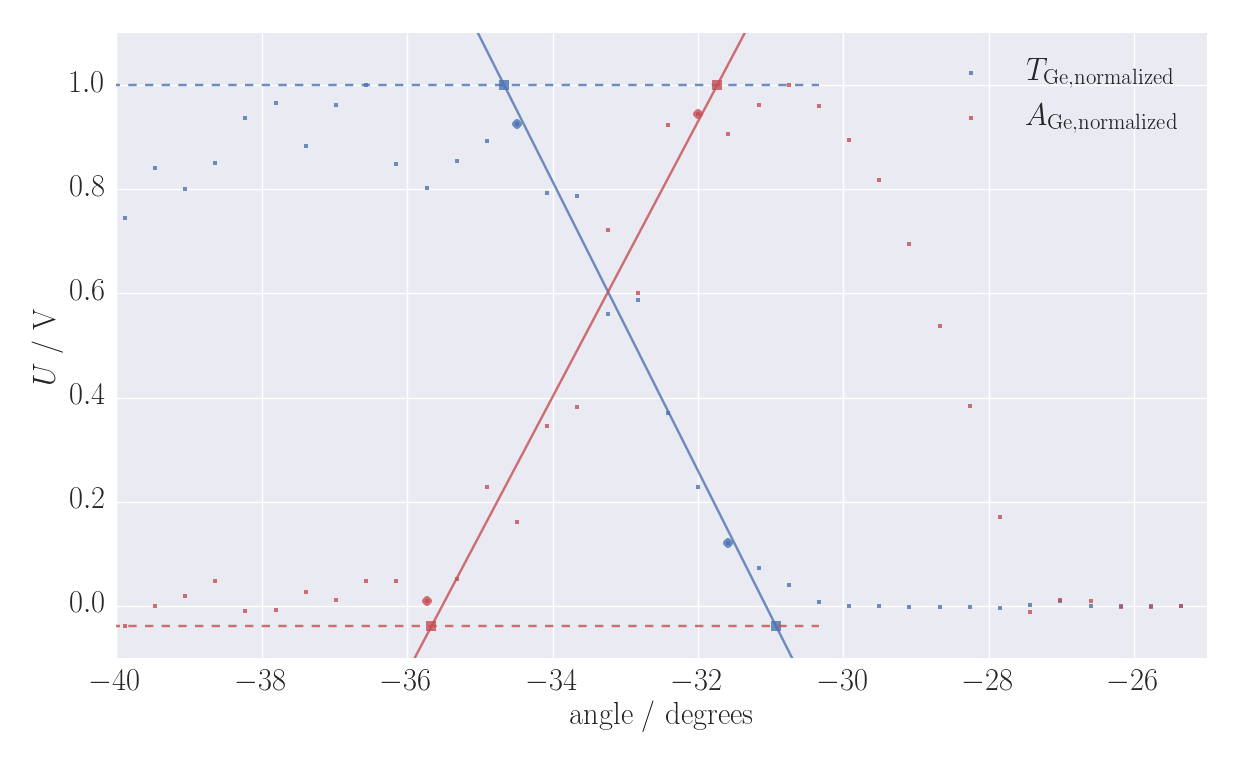
\includegraphics[width=1.0\linewidth]{figures/band_gap_result_Ge_left}
        \caption{}
        \label{fig:band_gap_result_Ge_left}
    \end{subfigure}
    \begin{subfigure}[b]{\pltw}
        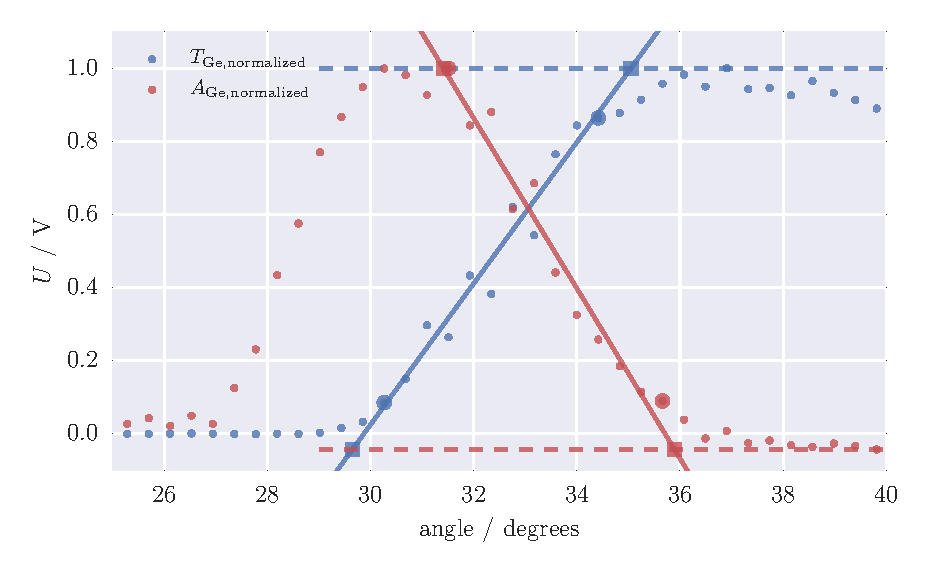
\includegraphics[width=1.0\linewidth]{figures/band_gap_result_Ge_right}
        \caption{}
        \label{fig:band_gap_result_Ge_right}
    \end{subfigure}
    \caption{
        Result of the procedure fitting straight lines through the points 
        at the transition from transmitting to absorbing characteristic
        for the Ge.
        For indications on the symbols, refer to figure 
        \ref{fig:band_gap_result_Si_left}. 
        }
    \label{fig:band_gap_result_Ge}
\end{figure}

\subsection{Raw data and gaussians for Haynes \& Shockley}
\label{sec:appendix_h_s_plots}
\begin{figure}
    \centering
    \begin{subfigure}[b]{\pltw}
        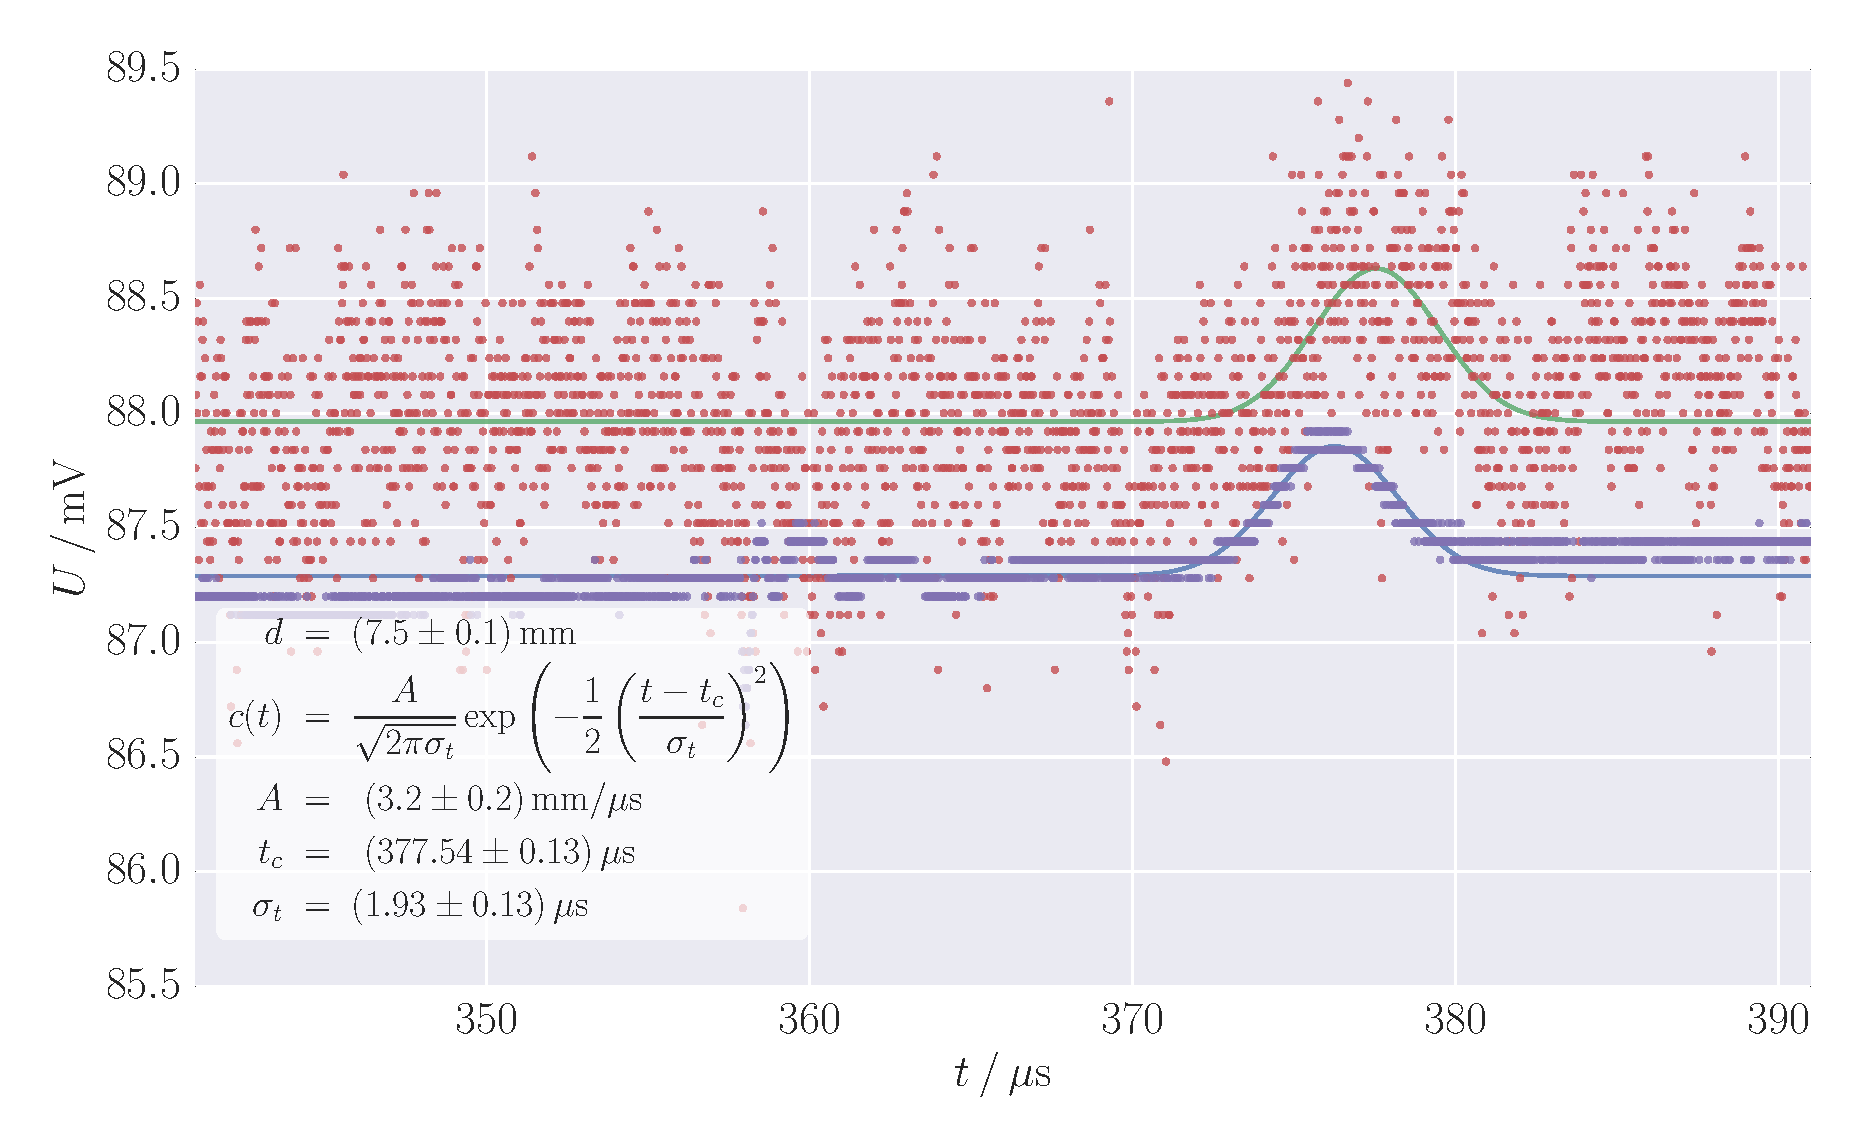
\includegraphics[width=1.0\linewidth]{figures/haynes_shockley_raw_10}
        \caption{}
        \label{fig:h_s_raw_10}
    \end{subfigure}
    \begin{subfigure}[b]{\pltw}
        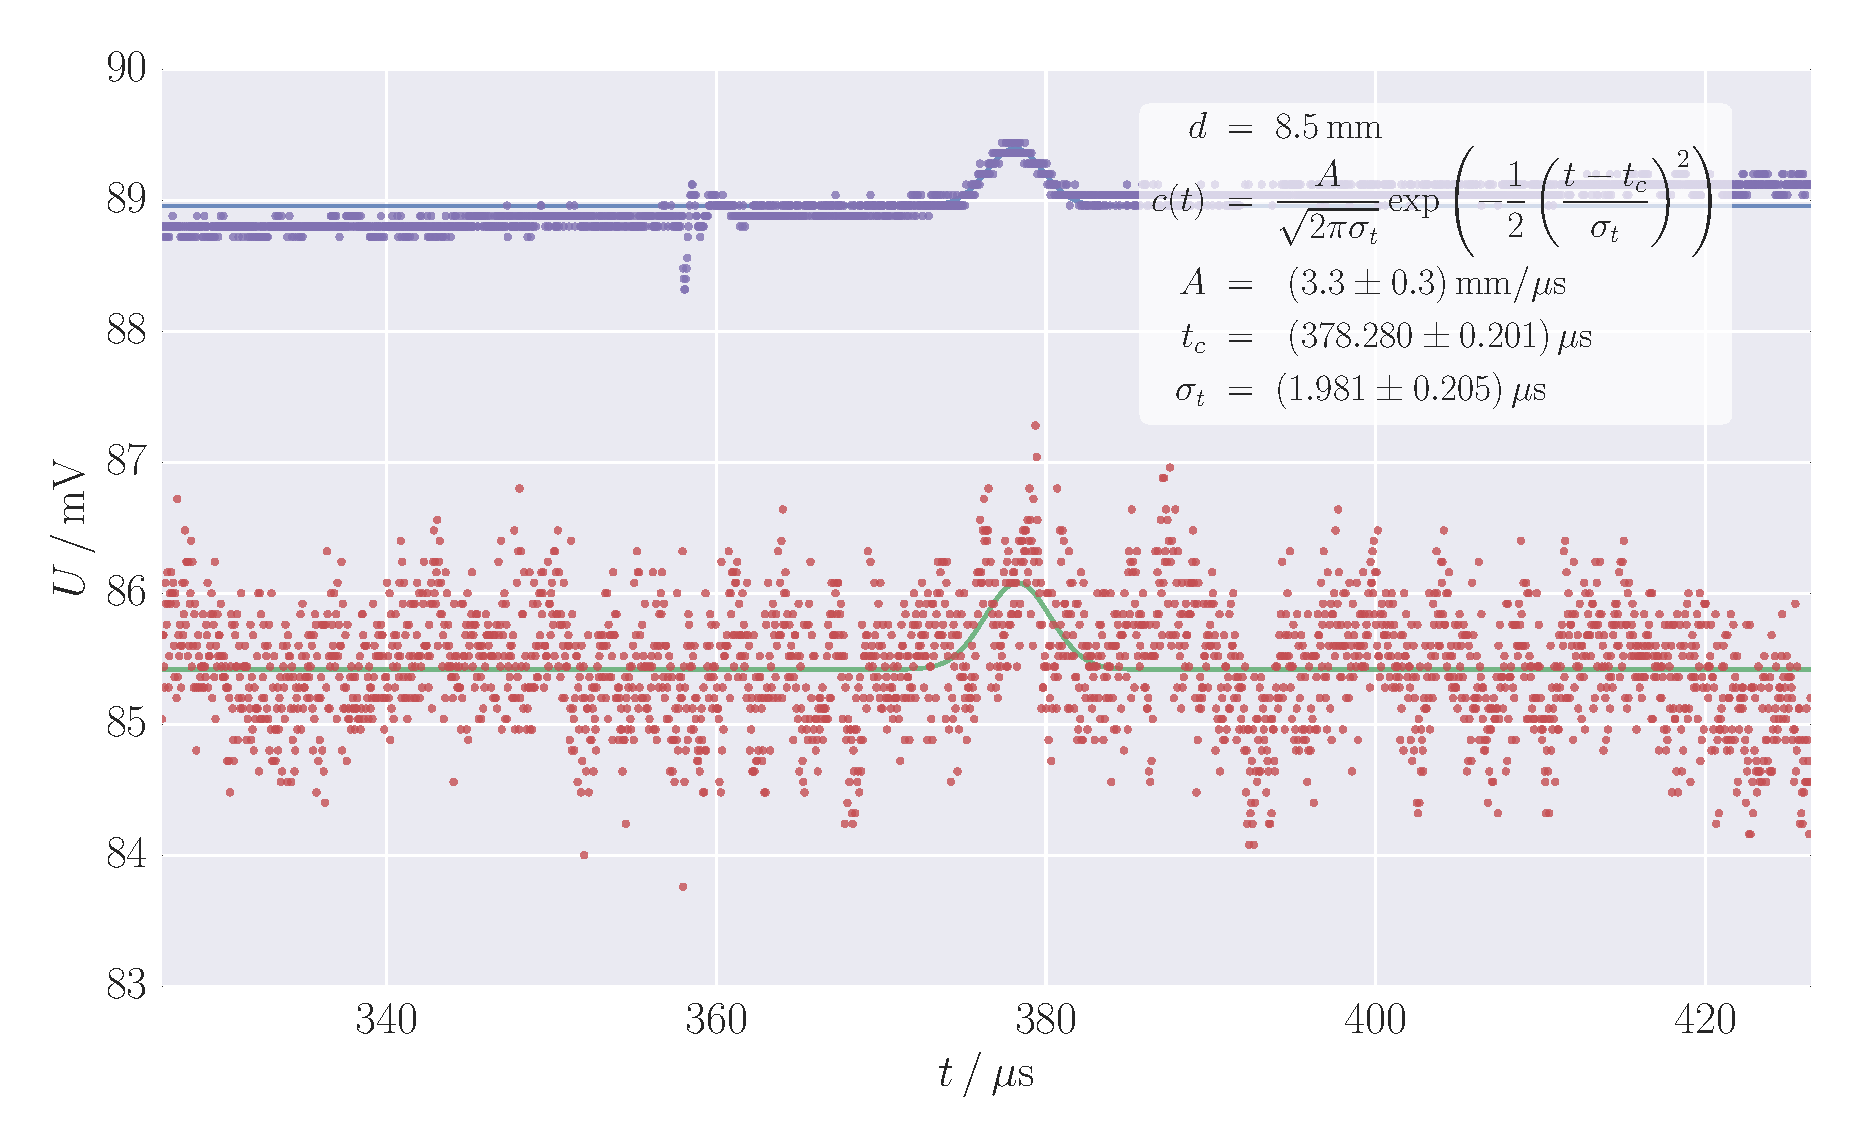
\includegraphics[width=1.0\linewidth]{figures/haynes_shockley_raw_12}
        \caption{}
        \label{fig:h_s_raw_12}
    \end{subfigure}
    \caption{
        Haynes \& Shockley experiment, measurement with constant $U$:
        Plots of raw data, averaged data and fitted gaussians. 
        The parameters of the gaussians are displayed in the boxes 
        ($c$ omitted).
        }
    \label{fig:h_s_raw_plots_10_12}
\end{figure}
\begin{figure}
    \centering
    \begin{subfigure}[b]{\pltw}
        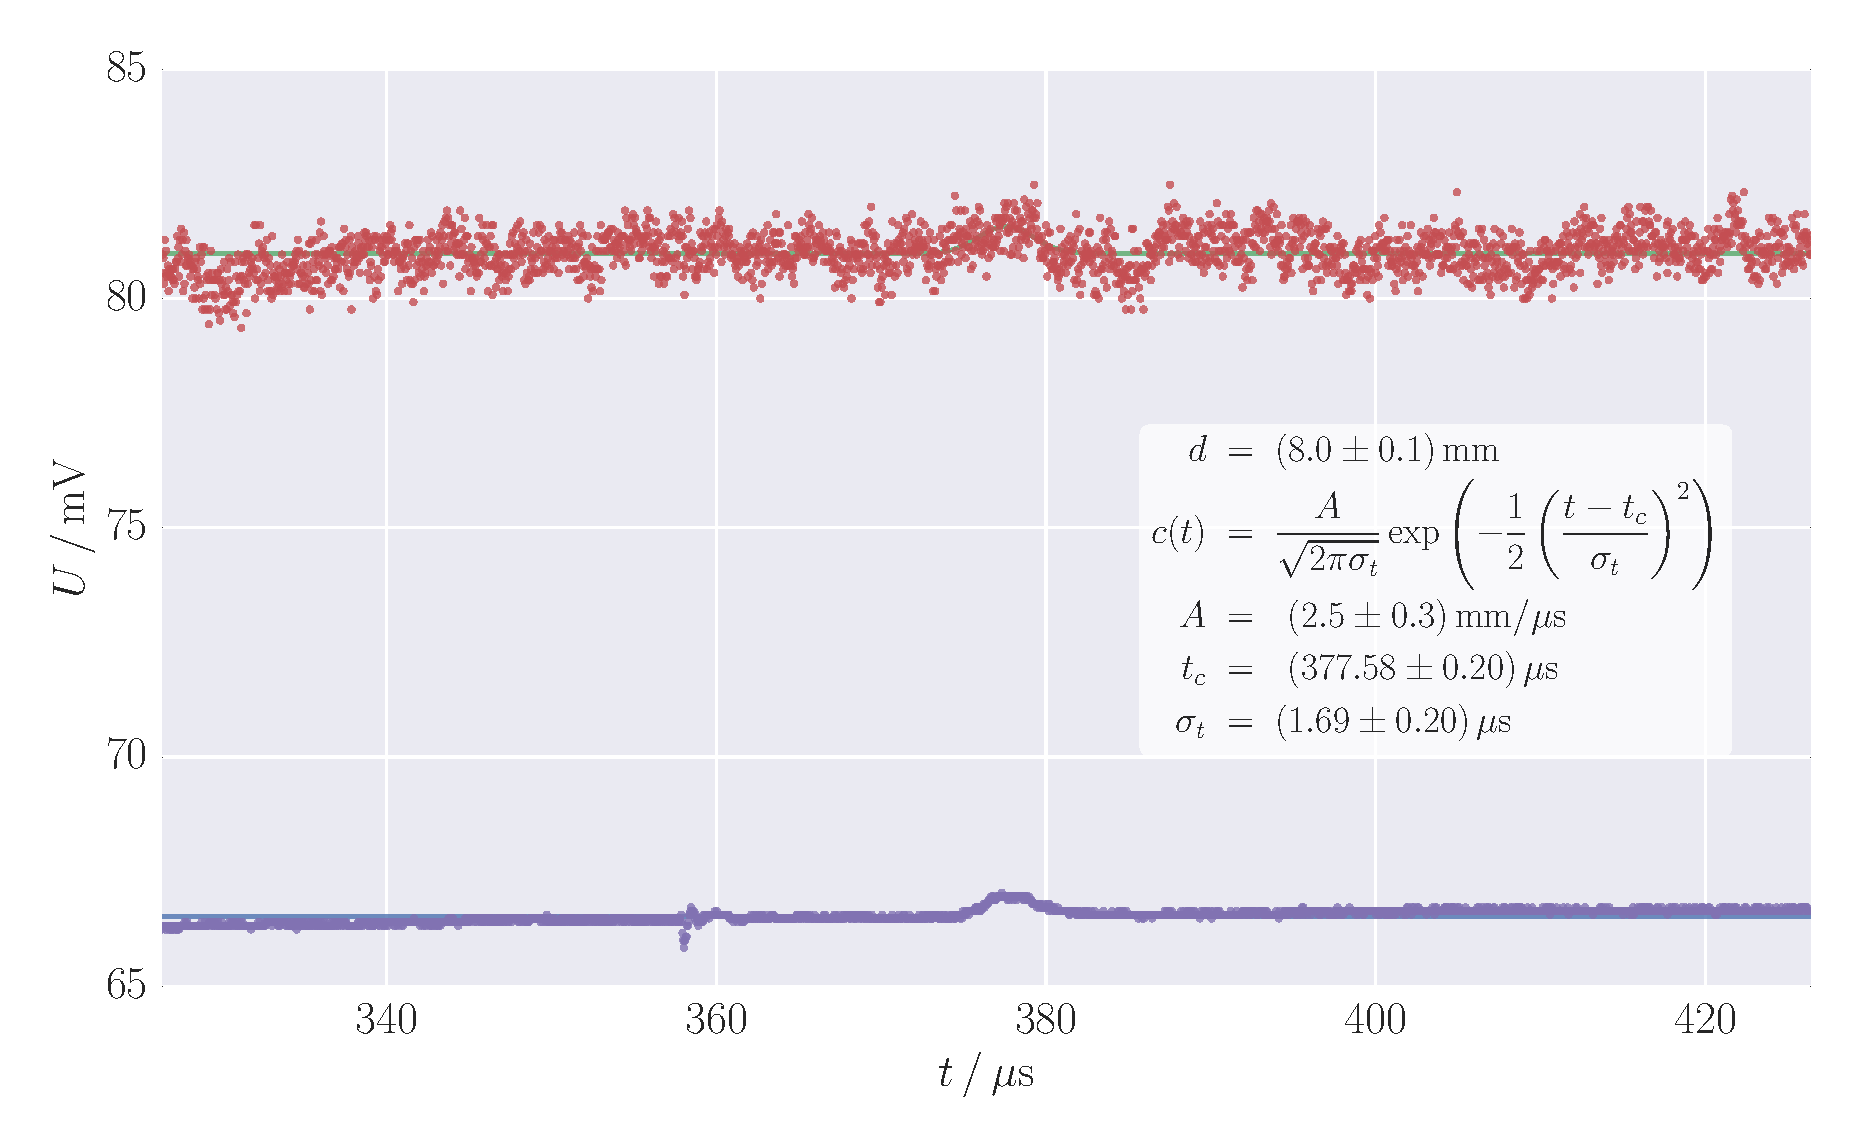
\includegraphics[width=1.0\linewidth]{figures/haynes_shockley_raw_17}
        \caption{}
        \label{fig:h_s_raw_17}
    \end{subfigure}
    \begin{subfigure}[b]{\pltw}
        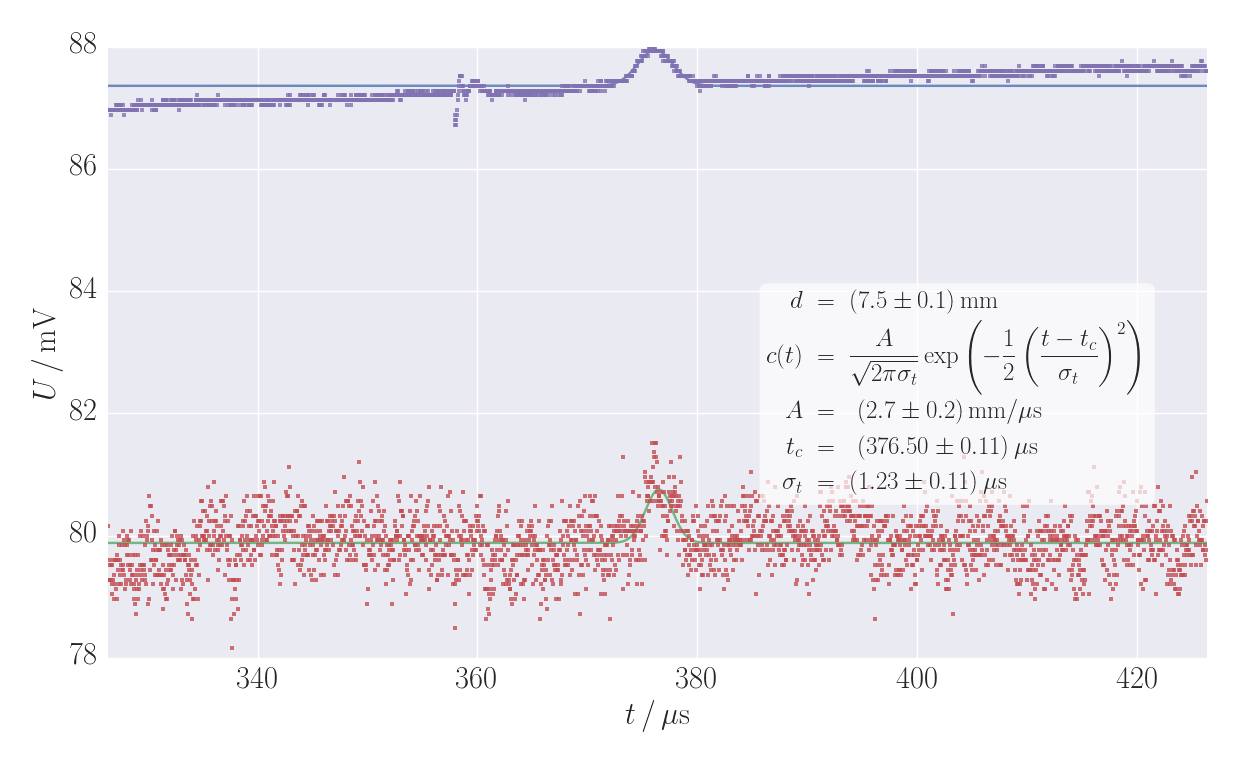
\includegraphics[width=1.0\linewidth]{figures/haynes_shockley_raw_18}
        \caption{}
        \label{fig:h_s_raw_18}
    \end{subfigure}
    \caption{
        (Continued)
        Haynes \& Shockley experiment, measurement with constant $U$:
        Plots of raw data, averaged data and fitted gaussians. 
        The parameters of the gaussians are displayed in the boxes 
        ($c$ omitted).
        }
    \label{fig:h_s_raw_plots_17_18}
\end{figure}
\begin{figure}
    \centering
    \begin{subfigure}[b]{\pltw}
        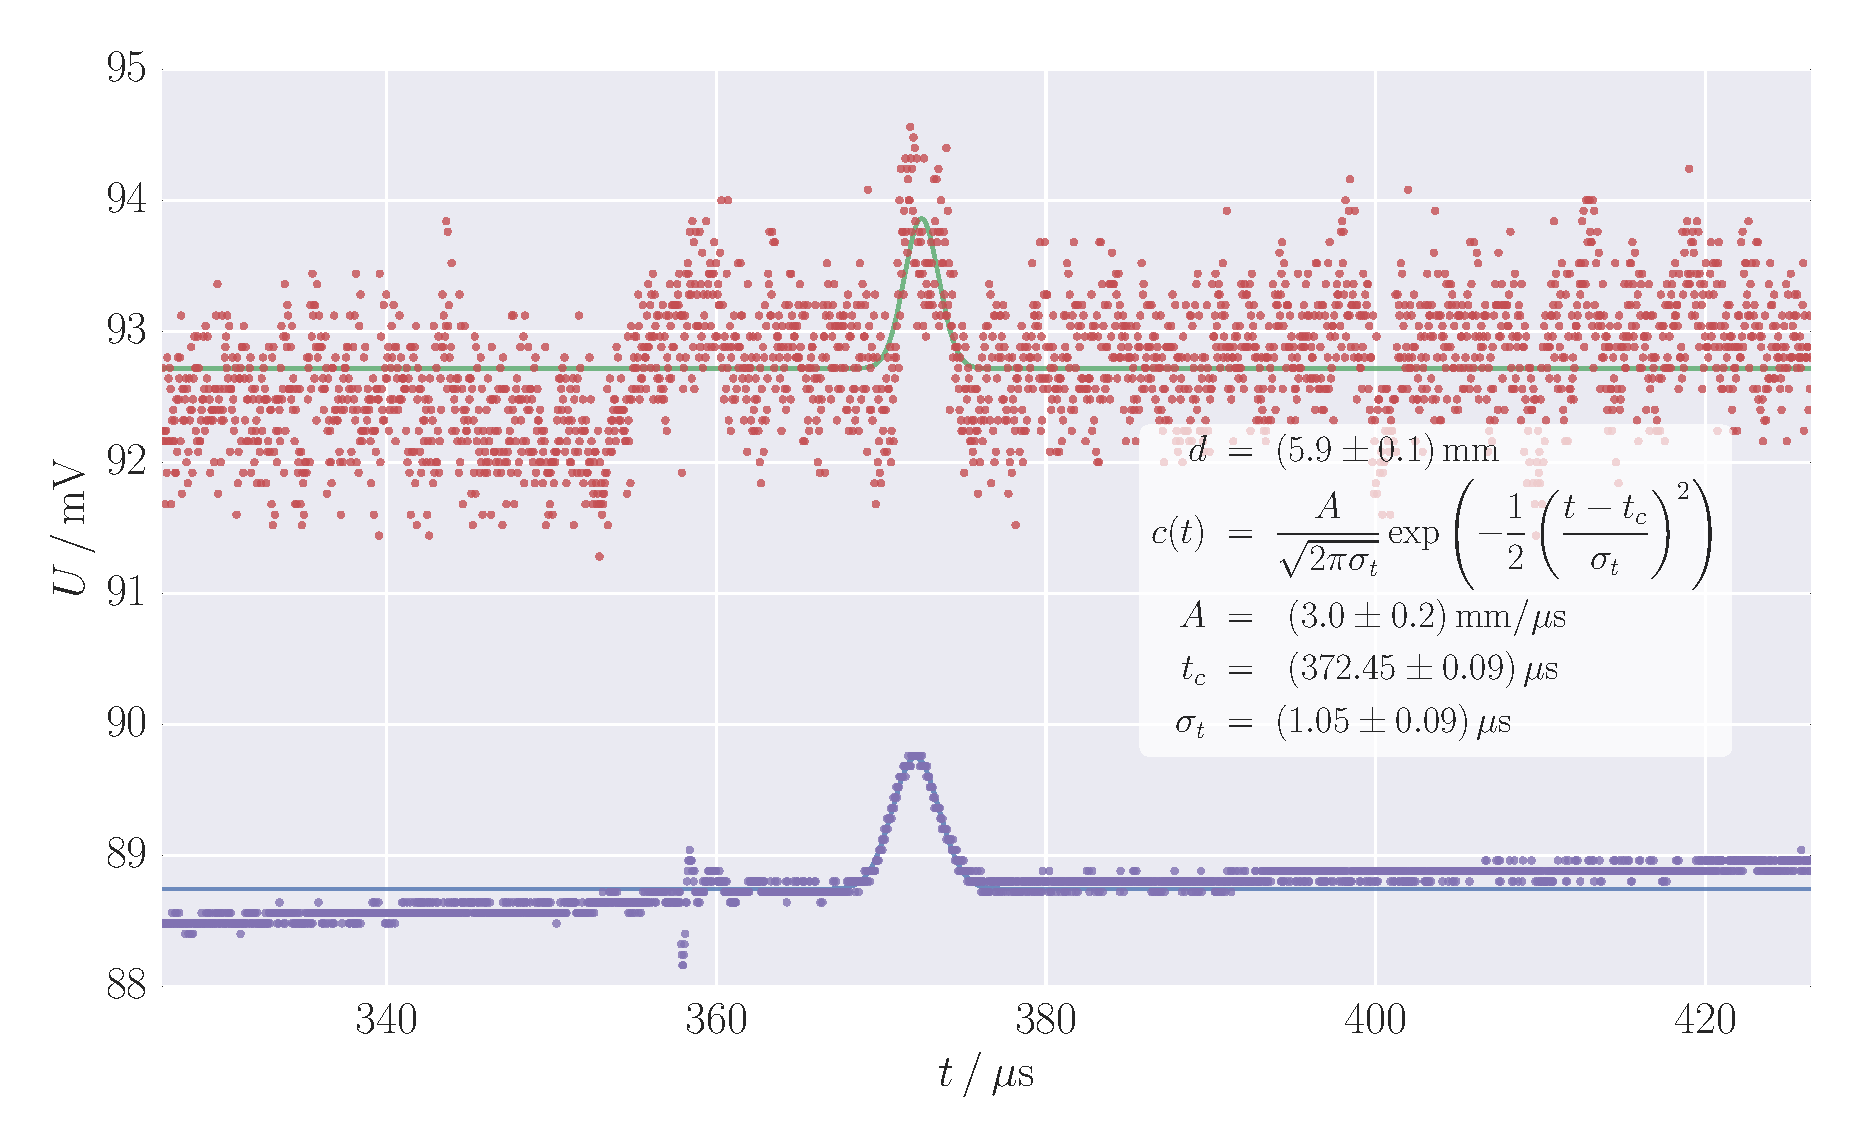
\includegraphics[width=1.0\linewidth]{figures/haynes_shockley_raw_22}
        \caption{}
        \label{fig:h_s_raw_22}
    \end{subfigure}
    \begin{subfigure}[b]{\pltw}
        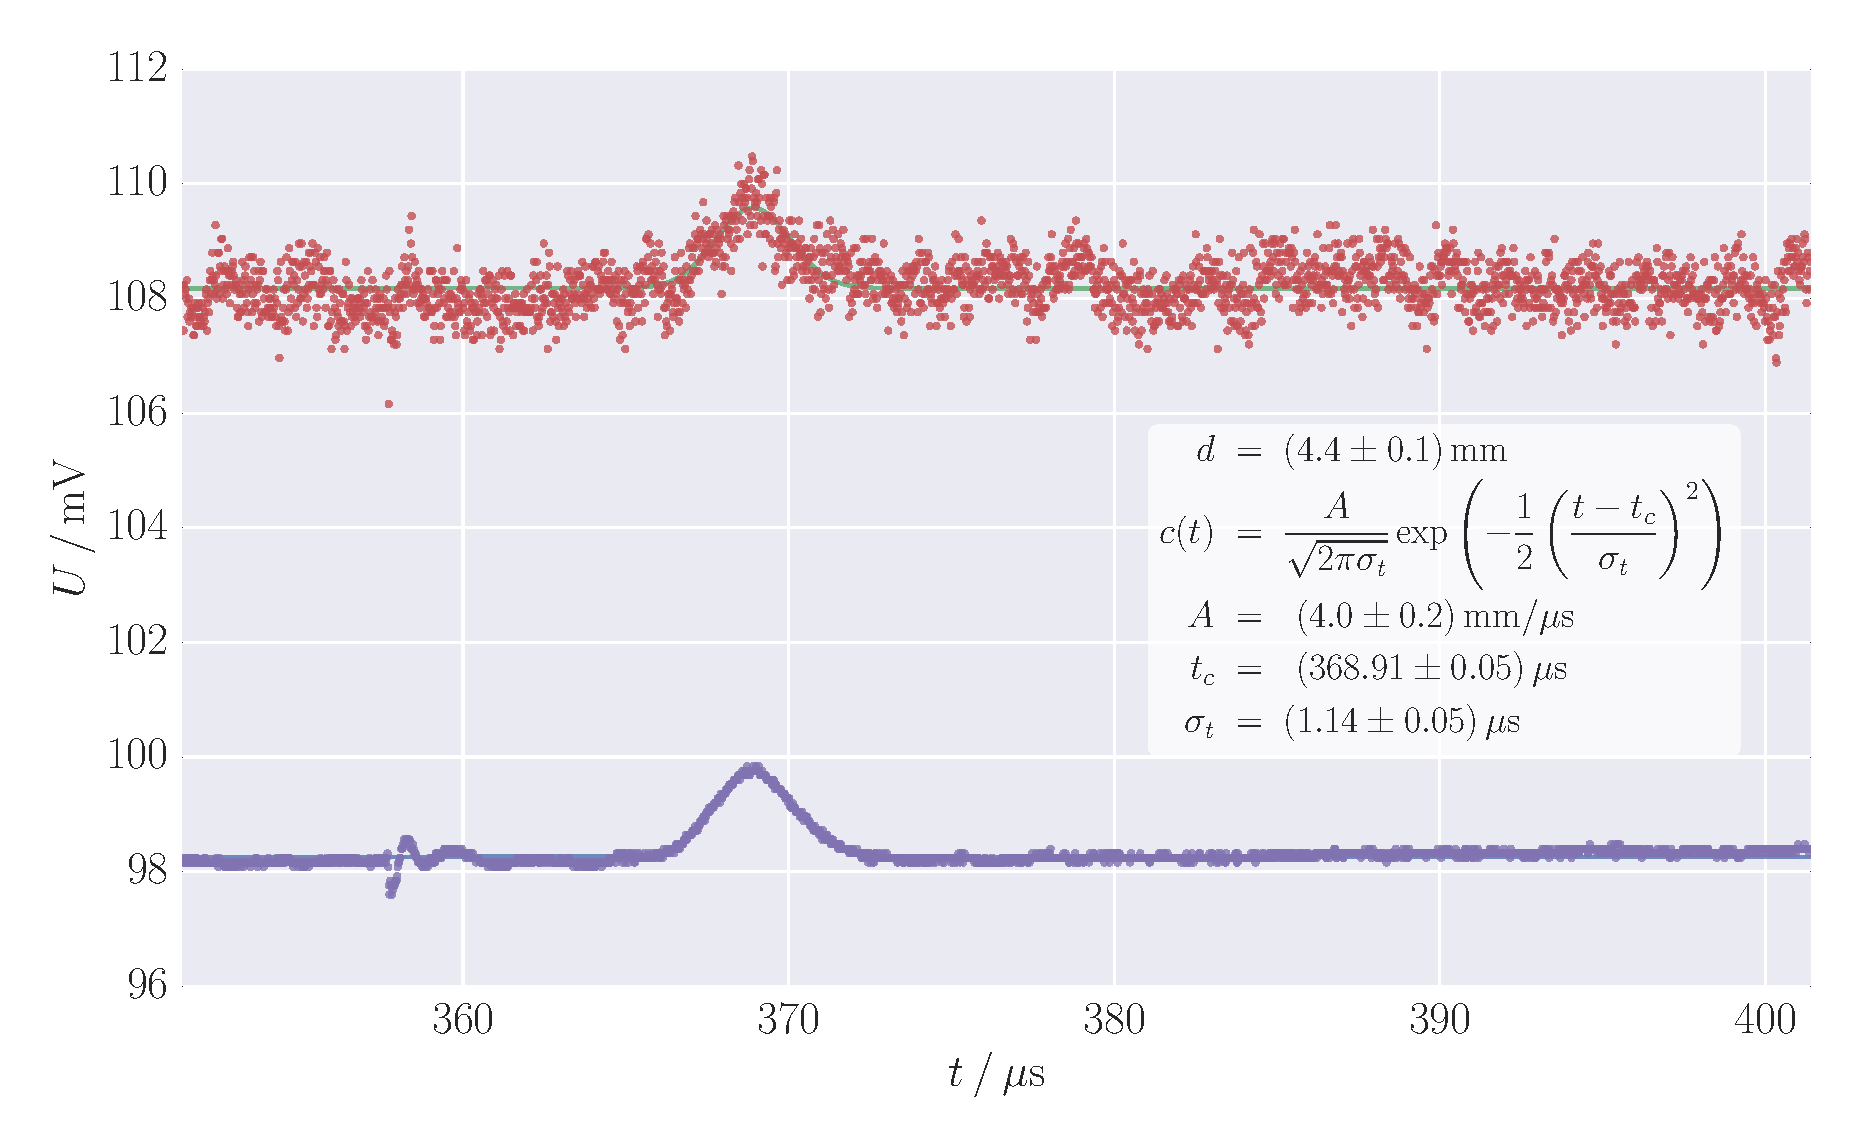
\includegraphics[width=1.0\linewidth]{figures/haynes_shockley_raw_24}
        \caption{}
        \label{fig:h_s_raw_24}
    \end{subfigure}
    \caption{
        (Continued)
        Haynes \& Shockley experiment, measurement with constant $U$:
        Plots of raw data, averaged data and fitted gaussians. 
        The parameters of the gaussians are displayed in the boxes 
        ($c$ omitted).
        }
    \label{fig:h_s_raw_plots_22_24}
\end{figure}
\begin{figure}
    \centering
    \begin{subfigure}[b]{\pltw}
        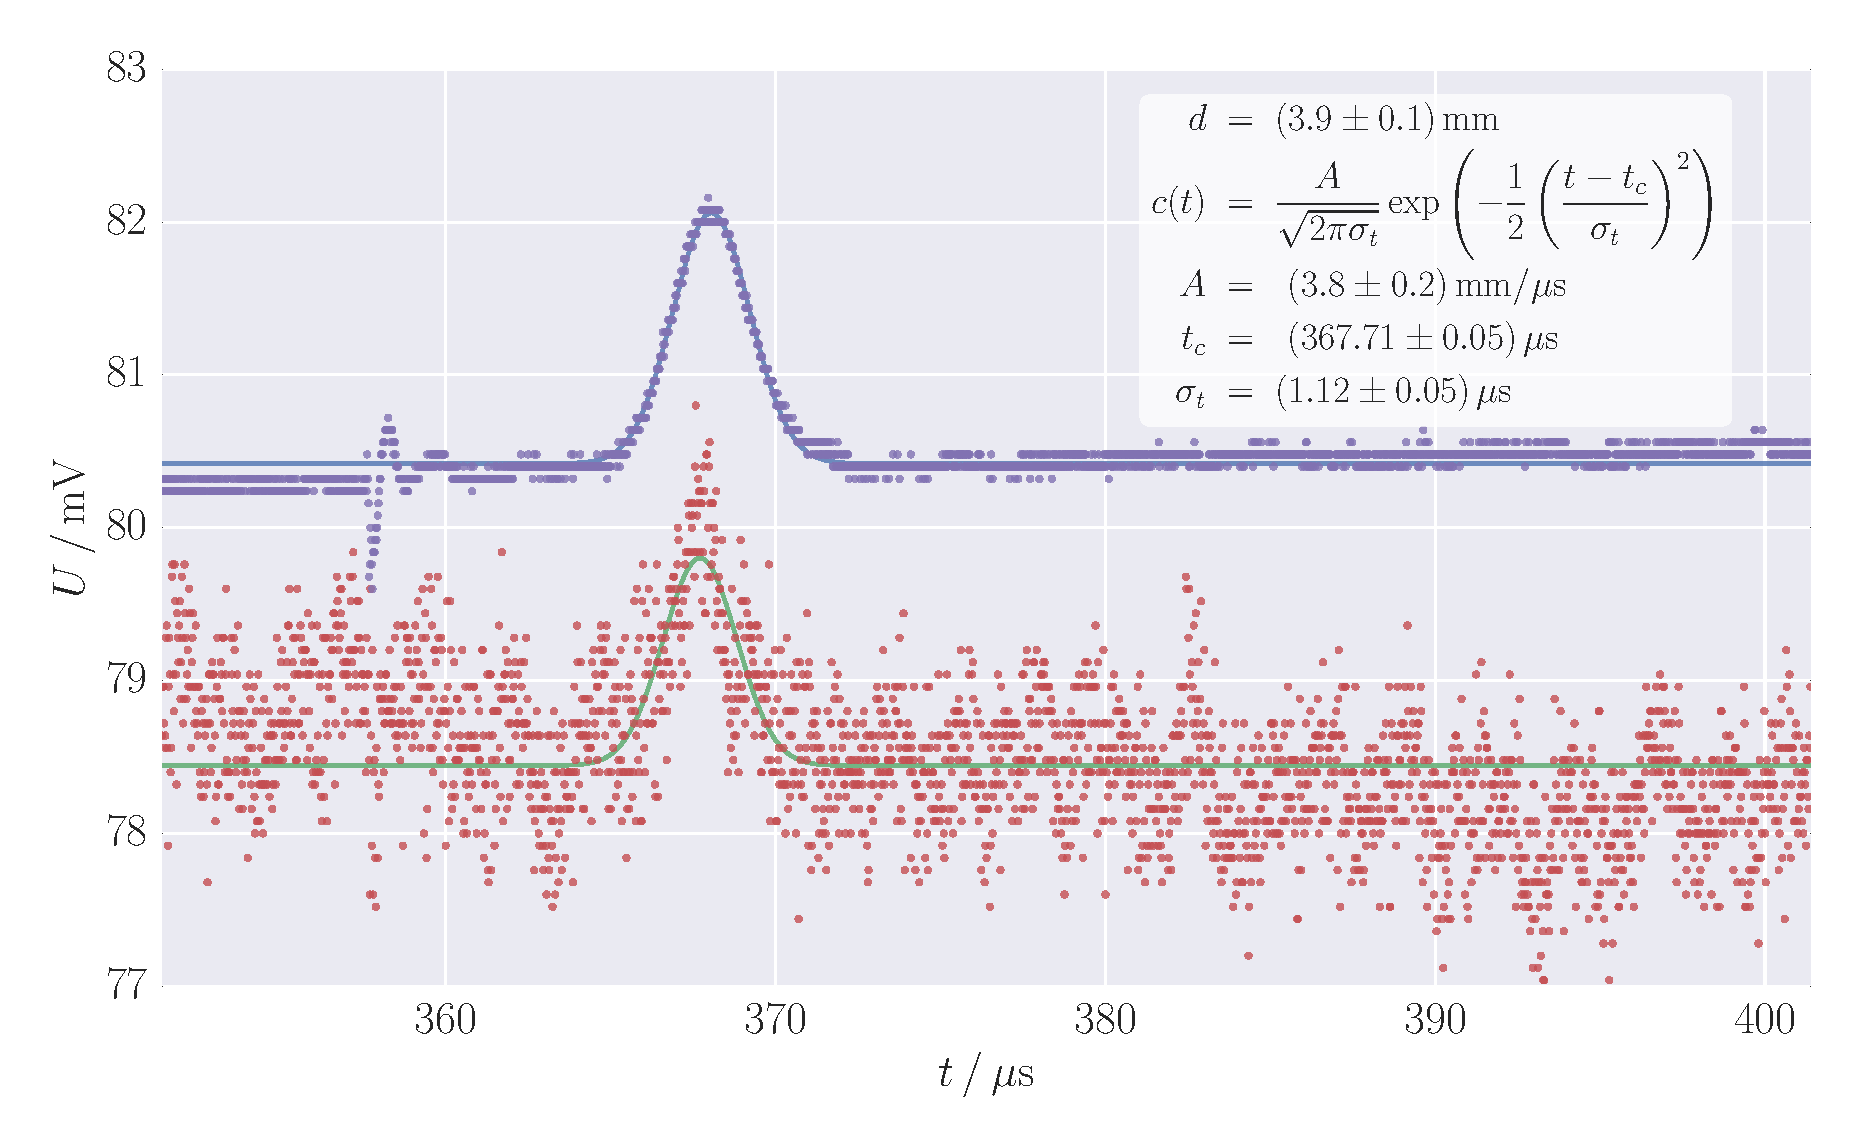
\includegraphics[width=1.0\linewidth]{figures/haynes_shockley_raw_26}
        \caption{}
        \label{fig:h_s_raw_26}
    \end{subfigure}
    \begin{subfigure}[b]{\pltw}
        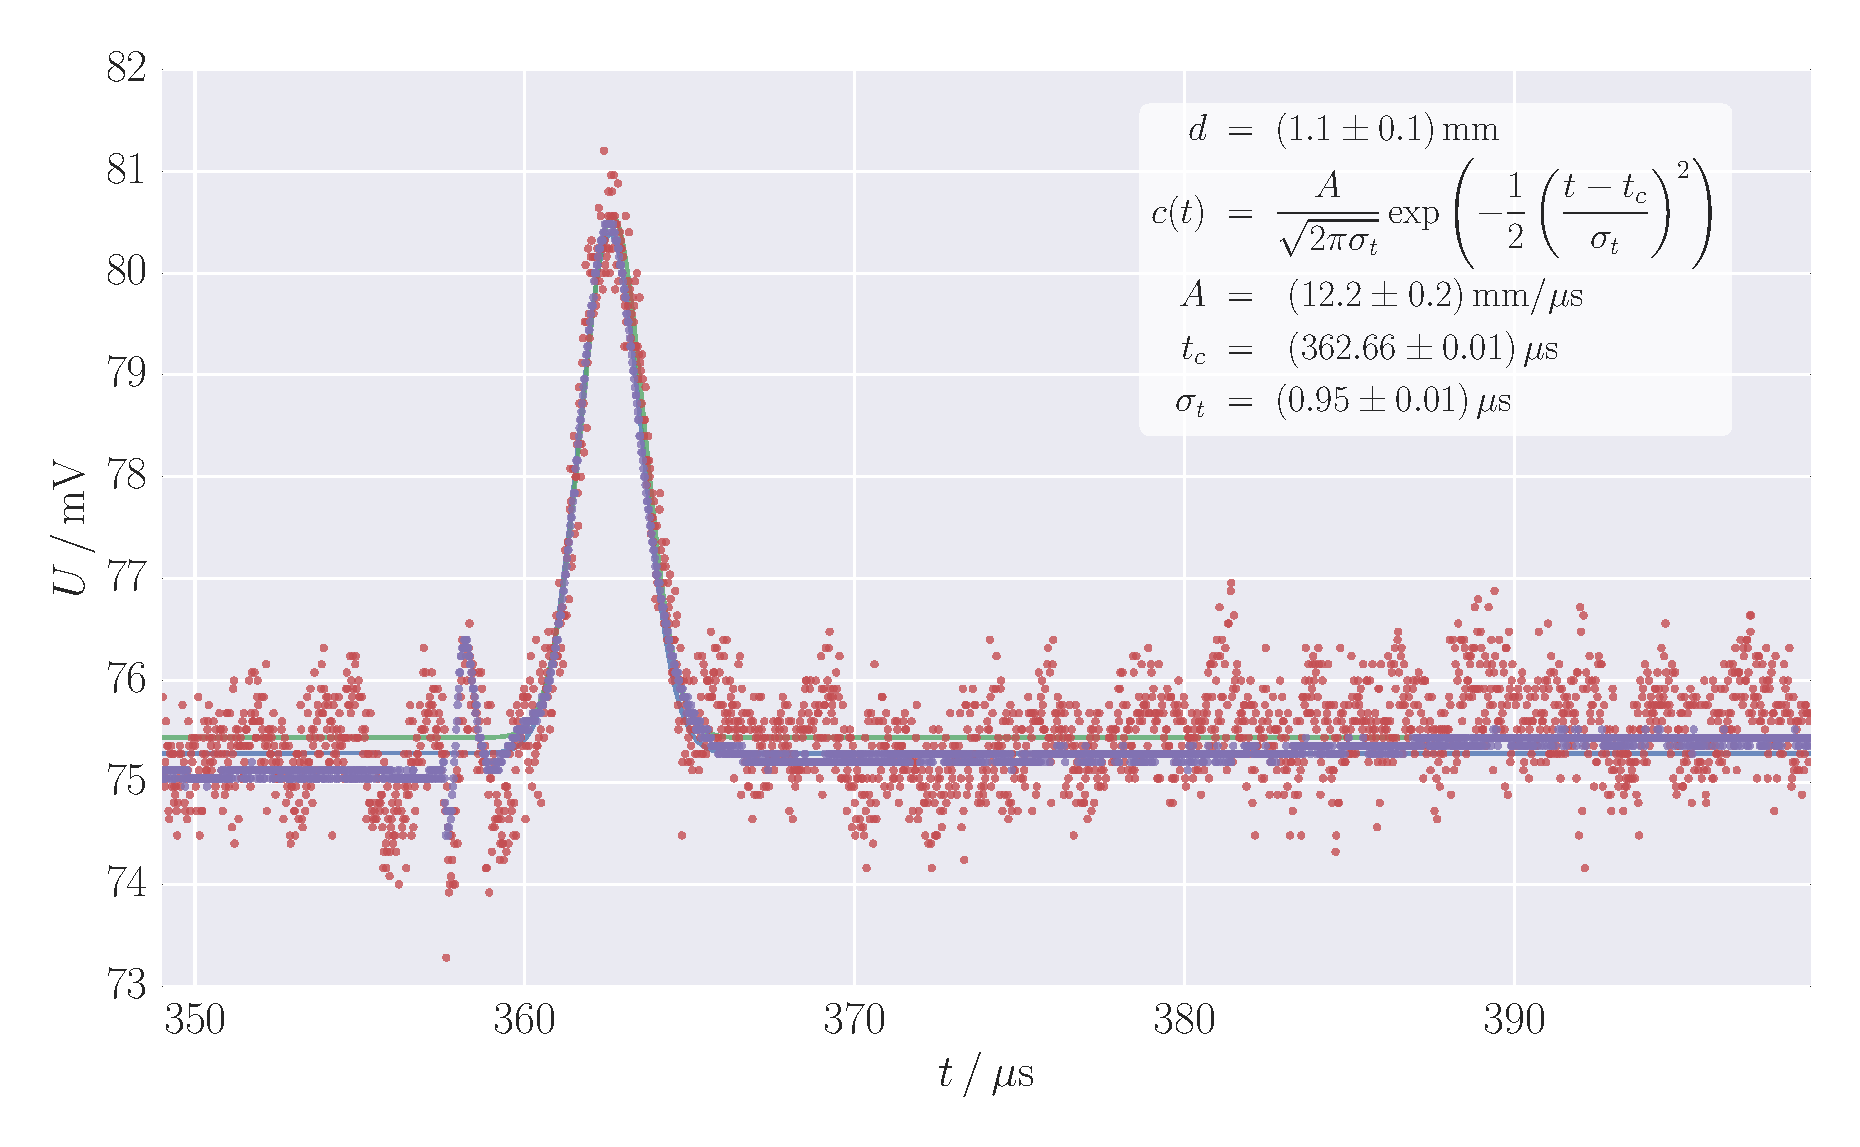
\includegraphics[width=1.0\linewidth]{figures/haynes_shockley_raw_33}
        \caption{}
        \label{fig:h_s_raw_33}
    \end{subfigure}
    \caption{
        (Continued)
        Haynes \& Shockley experiment, measurement with constant $U$:
        Plots of raw data, averaged data and fitted gaussians. 
        The parameters of the gaussians are displayed in the boxes 
        ($c$ omitted).
        }
    \label{fig:h_s_raw_plots_26_33}
\end{figure}
\label{sec:appendix_h_s_plots_U}
\begin{figure}
    \centering
    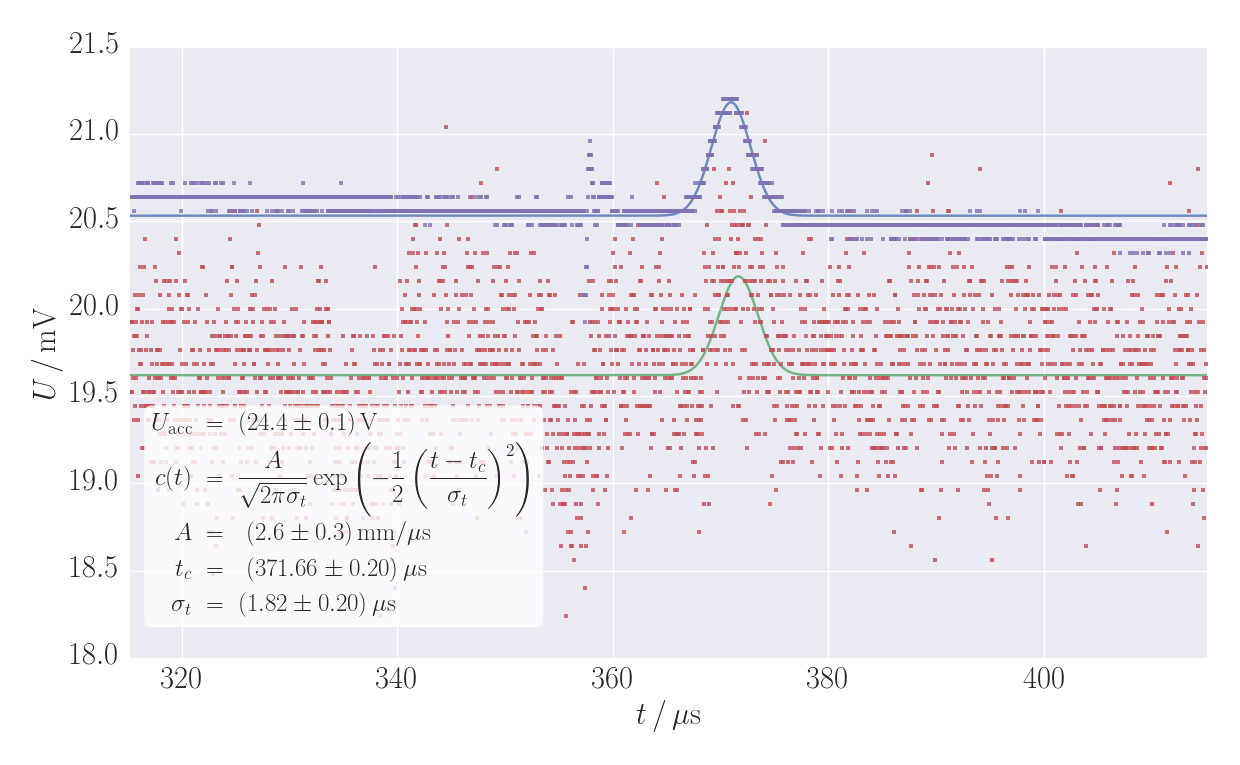
\includegraphics[width=1.0\textwidth]{figures/haynes_shockley_raw_U_59}
    \caption{
        Haynes \& Shockley experiment, measurement with constant $d$:
        Plots of raw data, averaged data and fitted gaussians. 
        The parameters of the gaussians are displayed in the boxes 
        ($c$ omitted). Here the raw data does not seem to show a signal. 
        However, the fitting algorithm did converge at the same point as 
        the smooth data. 
        }
    \label{fig:h_s_raw_U_59}
\end{figure}
\begin{figure}
    \centering
    \begin{subfigure}[b]{\pltw}
        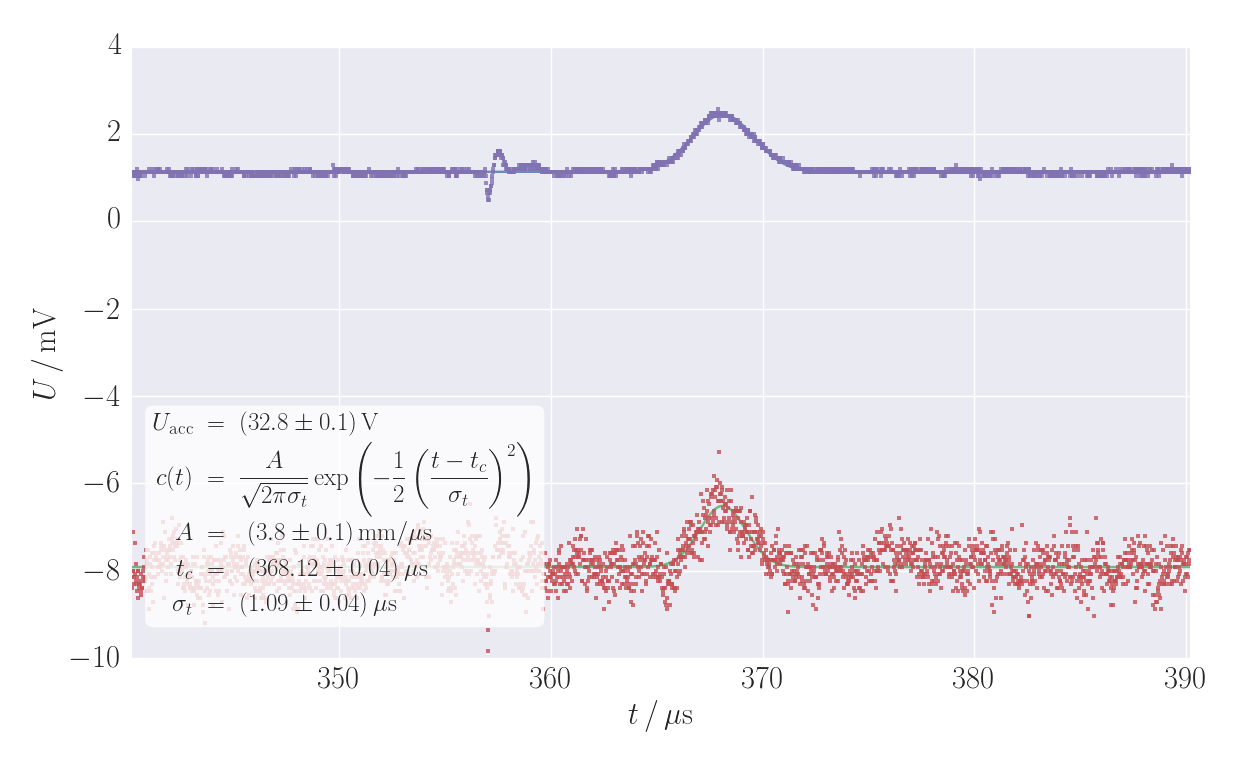
\includegraphics[width=1.0\linewidth]{figures/haynes_shockley_raw_U_61}
        \caption{}
        \label{fig:h_s_raw_U_61}
    \end{subfigure}
    \begin{subfigure}[b]{\pltw}
        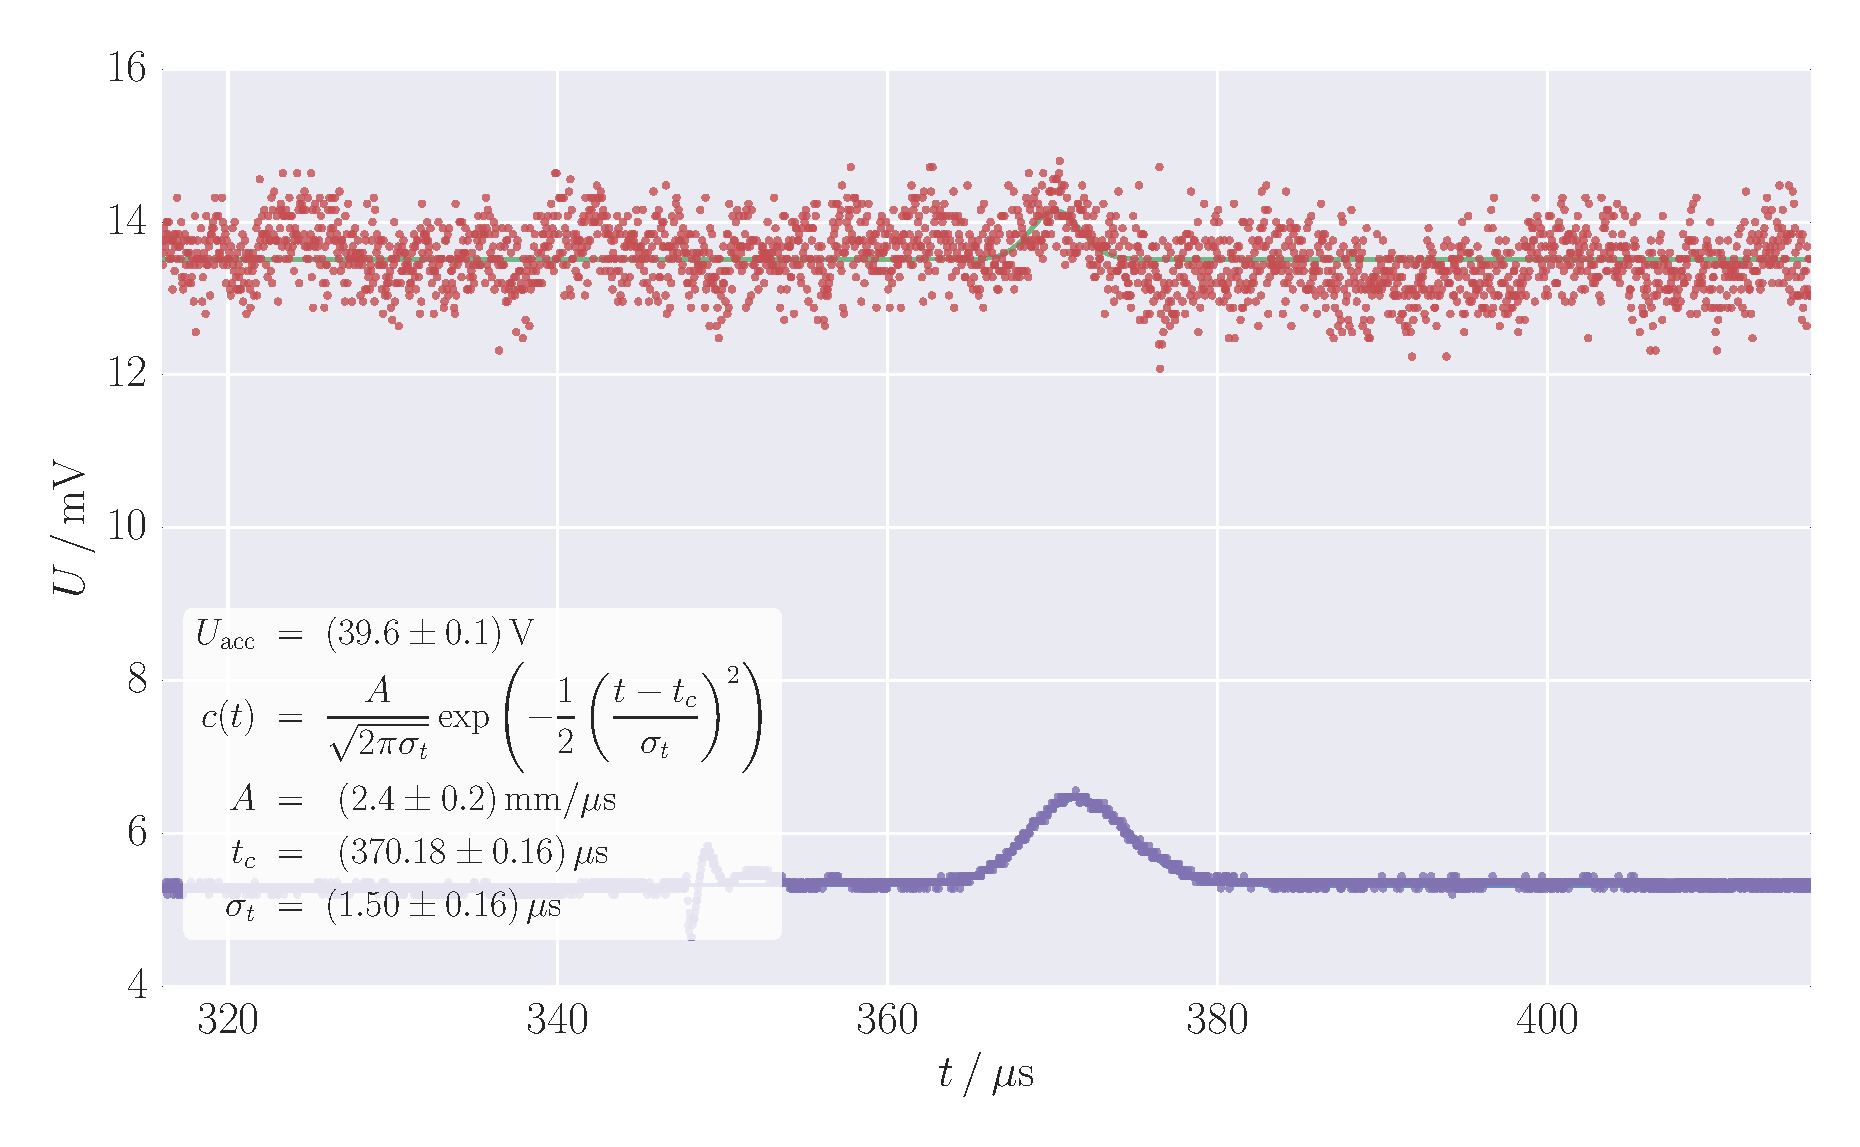
\includegraphics[width=1.0\linewidth]{figures/haynes_shockley_raw_U_47}
        \caption{}
        \label{fig:h_s_raw_U_47}
    \end{subfigure}
    \caption{
        Haynes \& Shockley experiment, measurement with constant $d$:
        Plots of raw data, averaged data and fitted gaussians. 
        The parameters of the gaussians are displayed in the boxes 
        ($c$ omitted).
        }
    \label{fig:h_s_raw_plots_U_61_47}
\end{figure}
\begin{figure}
    \centering
    \begin{subfigure}[b]{\pltw}
        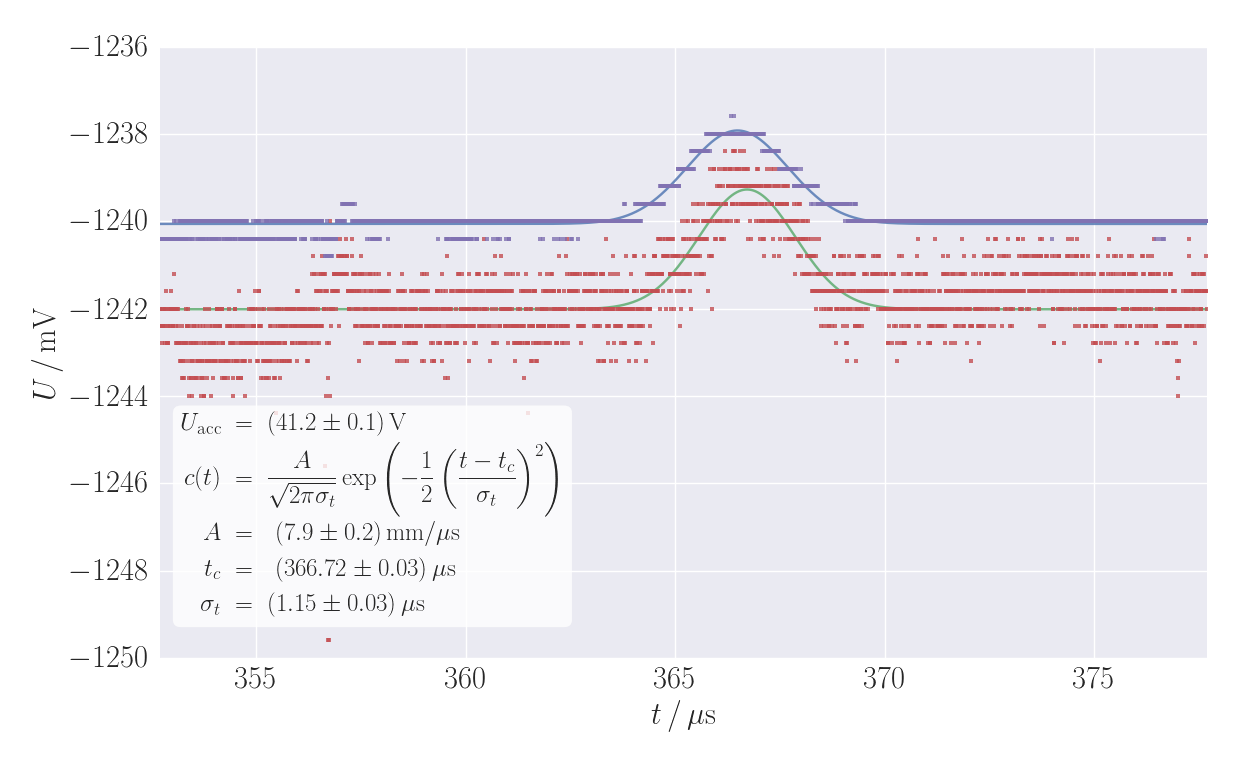
\includegraphics[width=1.0\linewidth]{figures/haynes_shockley_raw_U_63}
        \caption{}
        \label{fig:h_s_raw_U_63}
    \end{subfigure}
    \begin{subfigure}[b]{\pltw}
        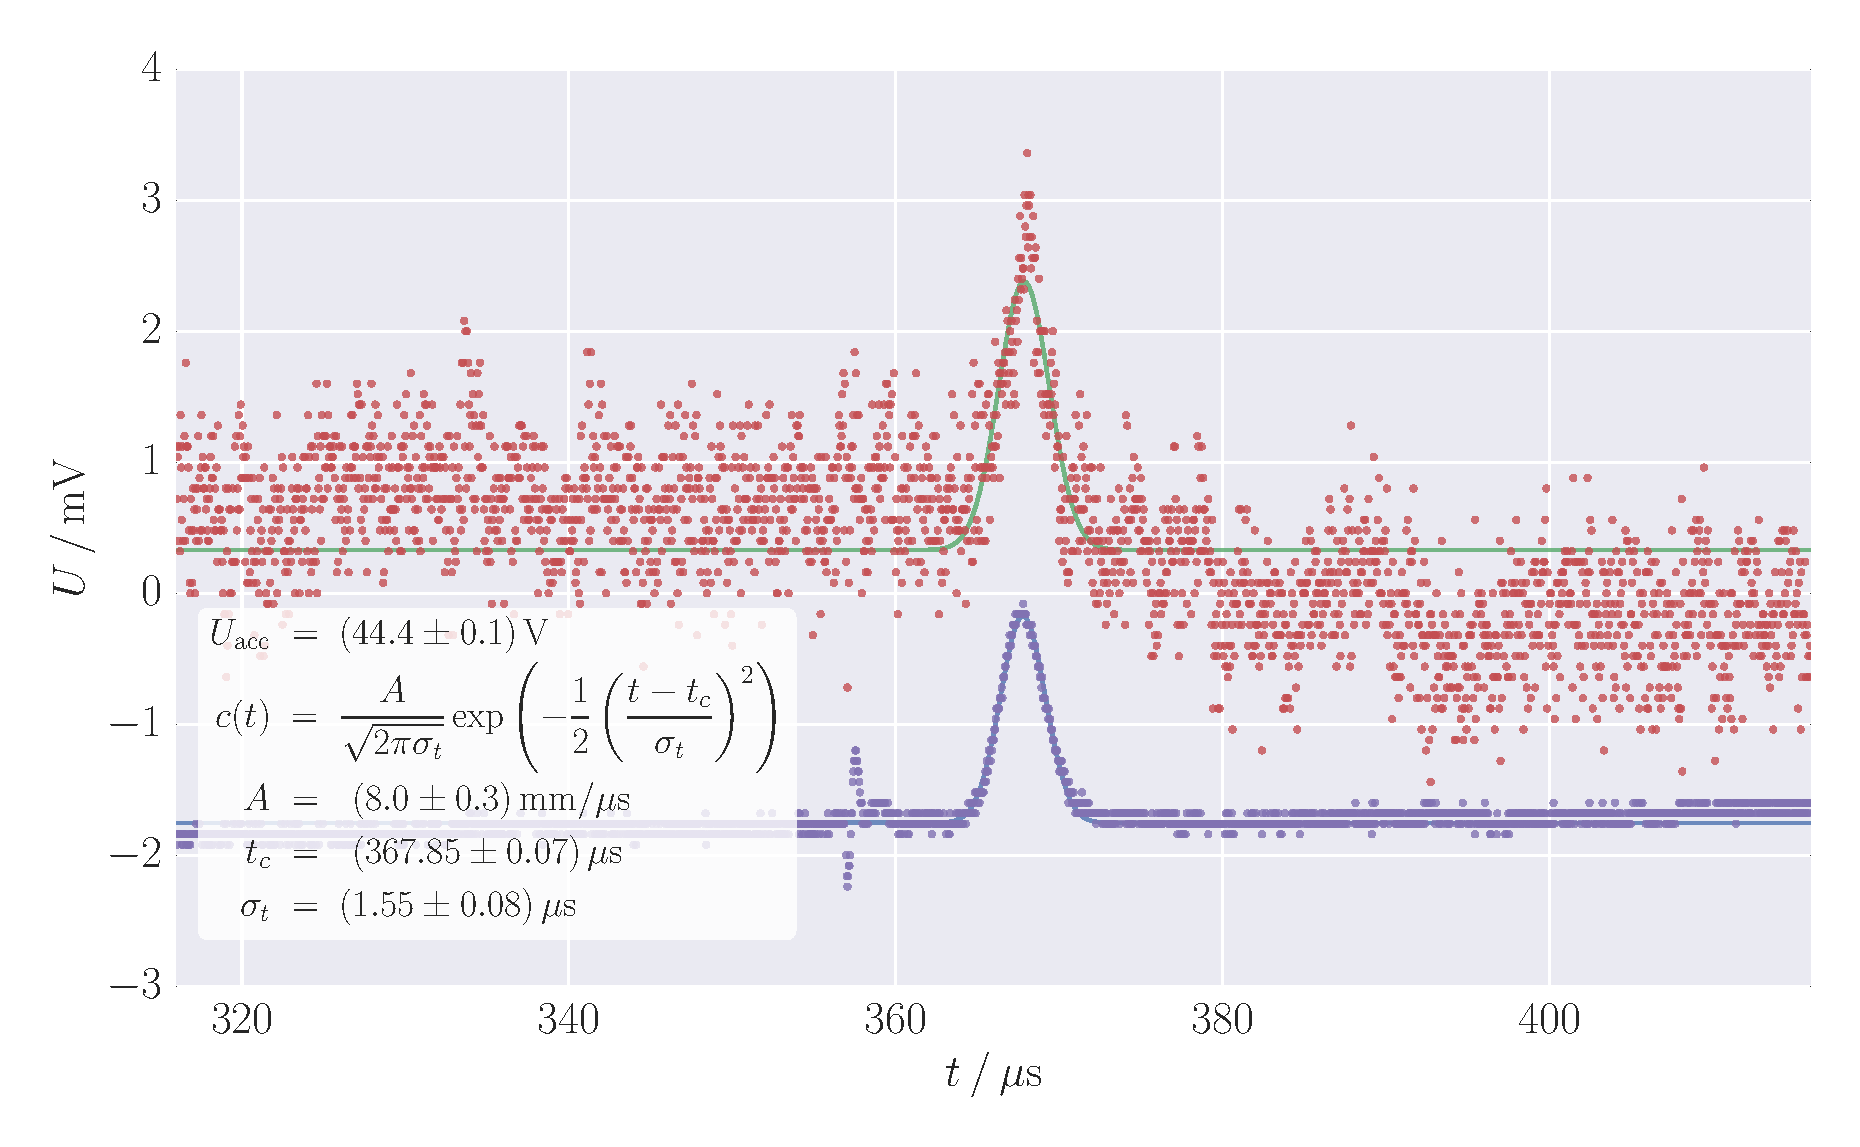
\includegraphics[width=1.0\linewidth]{figures/haynes_shockley_raw_U_43}
        \caption{}
        \label{fig:h_s_raw_U_43}
    \end{subfigure}
    \caption{
        (Continued)
        Haynes \& Shockley experiment, measurement with constant $d$:
        Plots of raw data, averaged data and fitted gaussians. 
        The parameters of the gaussians are displayed in the boxes 
        ($c$ omitted).
        }
    \label{fig:h_s_raw_plots_U_63_43}
\end{figure}
\begin{figure}
    \centering
    \begin{subfigure}[b]{\pltw}
        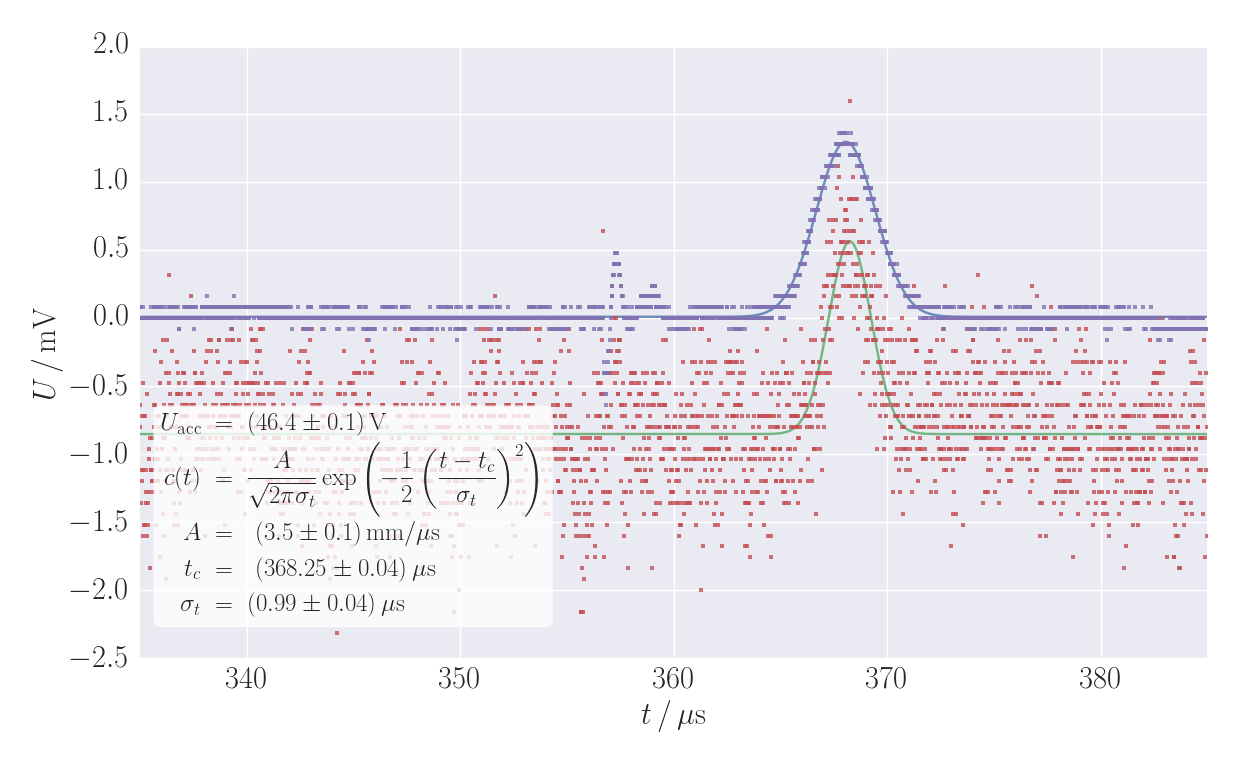
\includegraphics[width=1.0\linewidth]{figures/haynes_shockley_raw_U_67}
        \caption{}
        \label{fig:h_s_raw_U_67}
    \end{subfigure}
    \begin{subfigure}[b]{\pltw}
        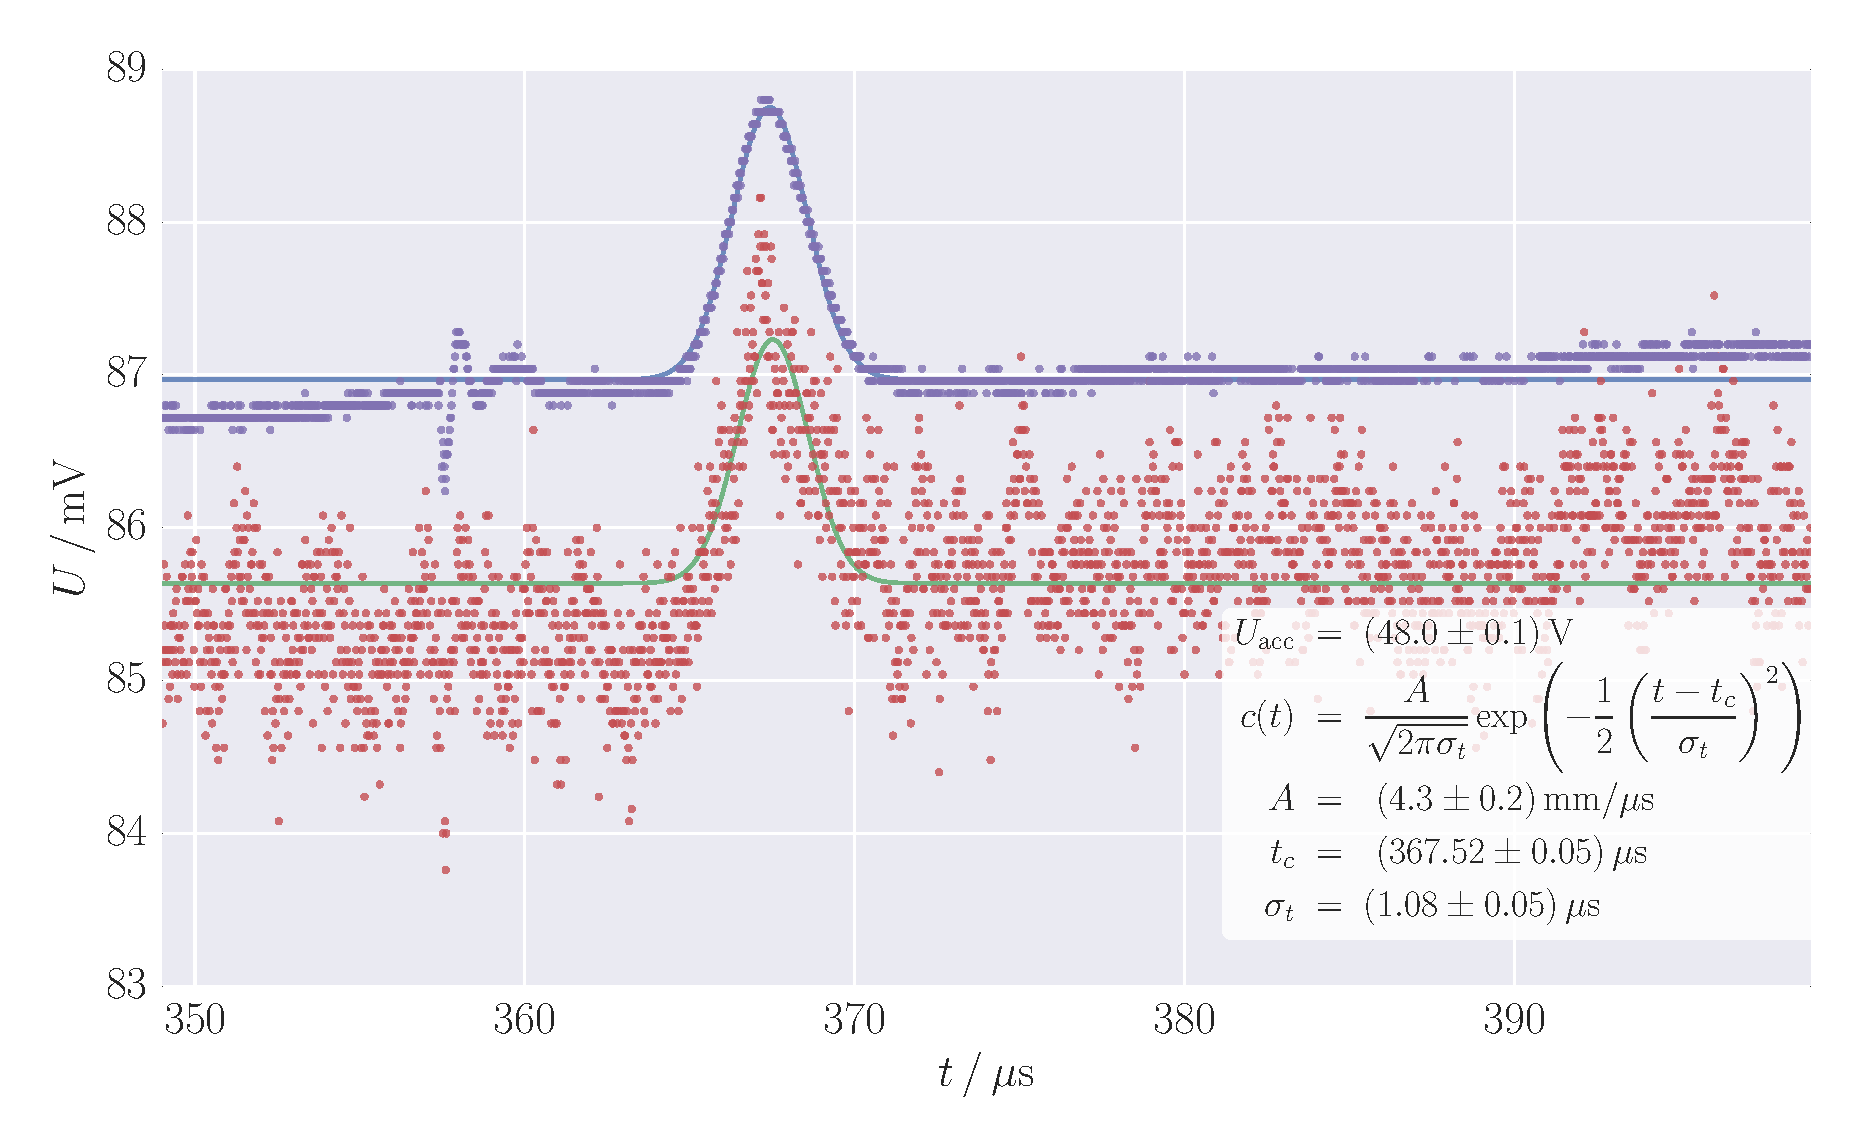
\includegraphics[width=1.0\linewidth]{figures/haynes_shockley_raw_U_35}
        \caption{}
        \label{fig:h_s_raw_U_35}
    \end{subfigure}
    \caption{
        (Continued)
        Haynes \& Shockley experiment, measurement with constant $d$:
        Plots of raw data, averaged data and fitted gaussians. 
        The parameters of the gaussians are displayed in the boxes 
        ($c$ omitted).
        }
    \label{fig:h_s_raw_plots_U_67_35}
\end{figure}
\begin{figure}
    \centering
    \begin{subfigure}[b]{\pltw}
        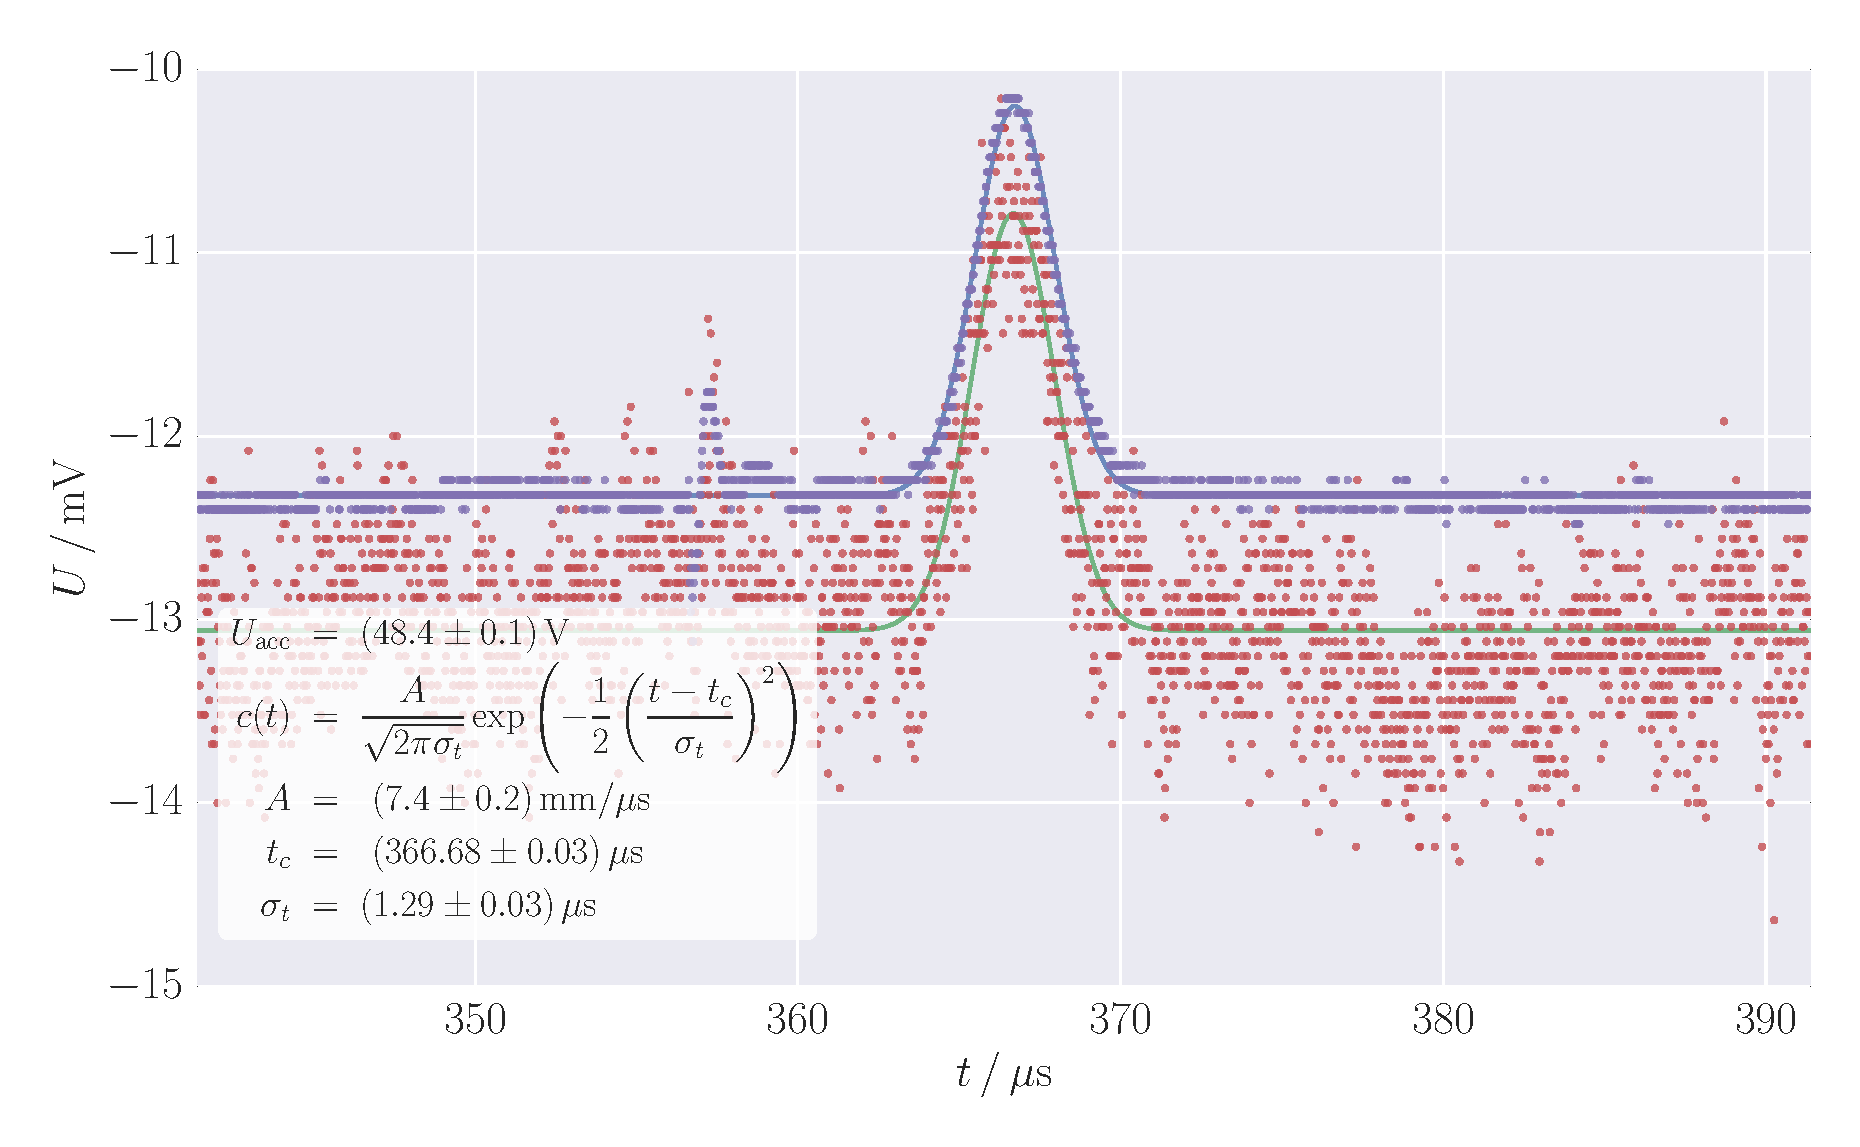
\includegraphics[width=1.0\linewidth]{figures/haynes_shockley_raw_U_39}
        \caption{}
        \label{fig:h_s_raw_U_39}
    \end{subfigure}
    \begin{subfigure}[b]{\pltw}
        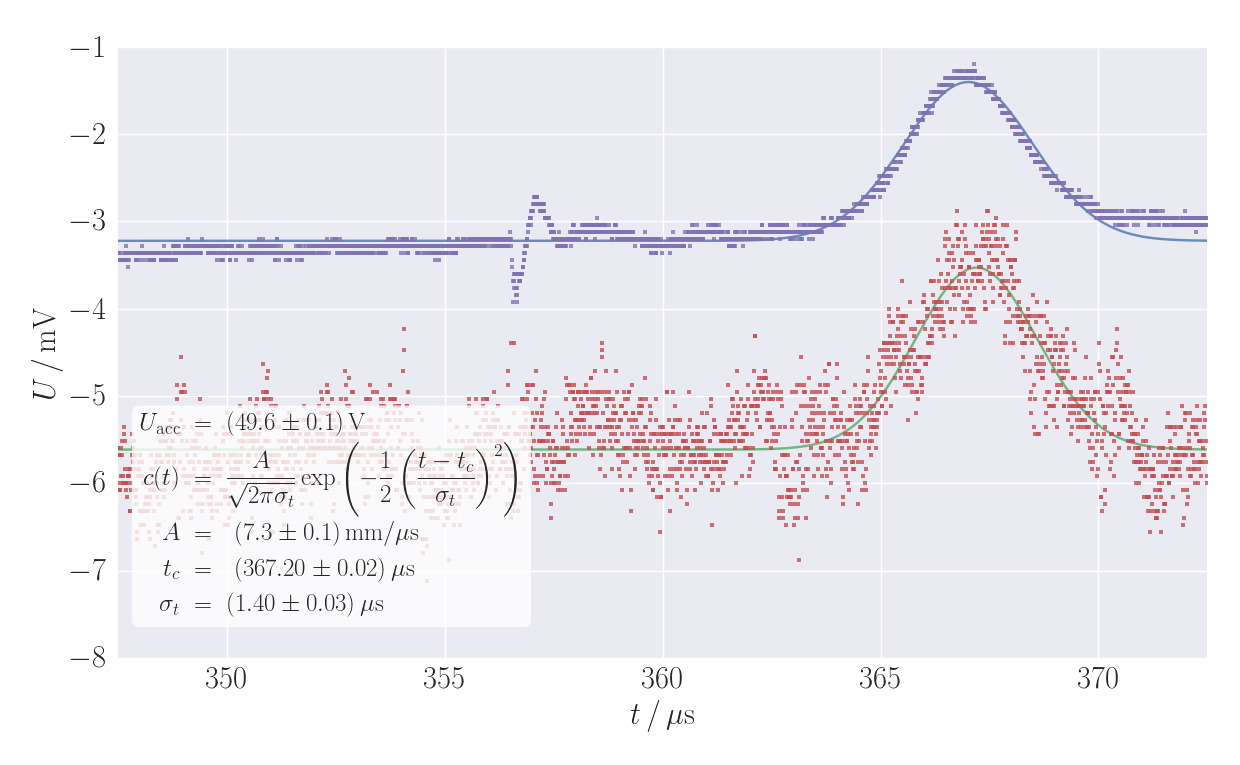
\includegraphics[width=1.0\linewidth]{figures/haynes_shockley_raw_U_65}
        \caption{}
        \label{fig:h_s_raw_U_65}
    \end{subfigure}
    \caption{
        (Continued)
        Haynes \& Shockley experiment, measurement with constant $d$:
        Plots of raw data, averaged data and fitted gaussians. 
        The parameters of the gaussians are displayed in the boxes 
        ($c$ omitted).
        }
    \label{fig:h_s_raw_plots_U_39_65}
\end{figure}
\begin{figure}
    \centering
    \begin{subfigure}[b]{\pltw}
        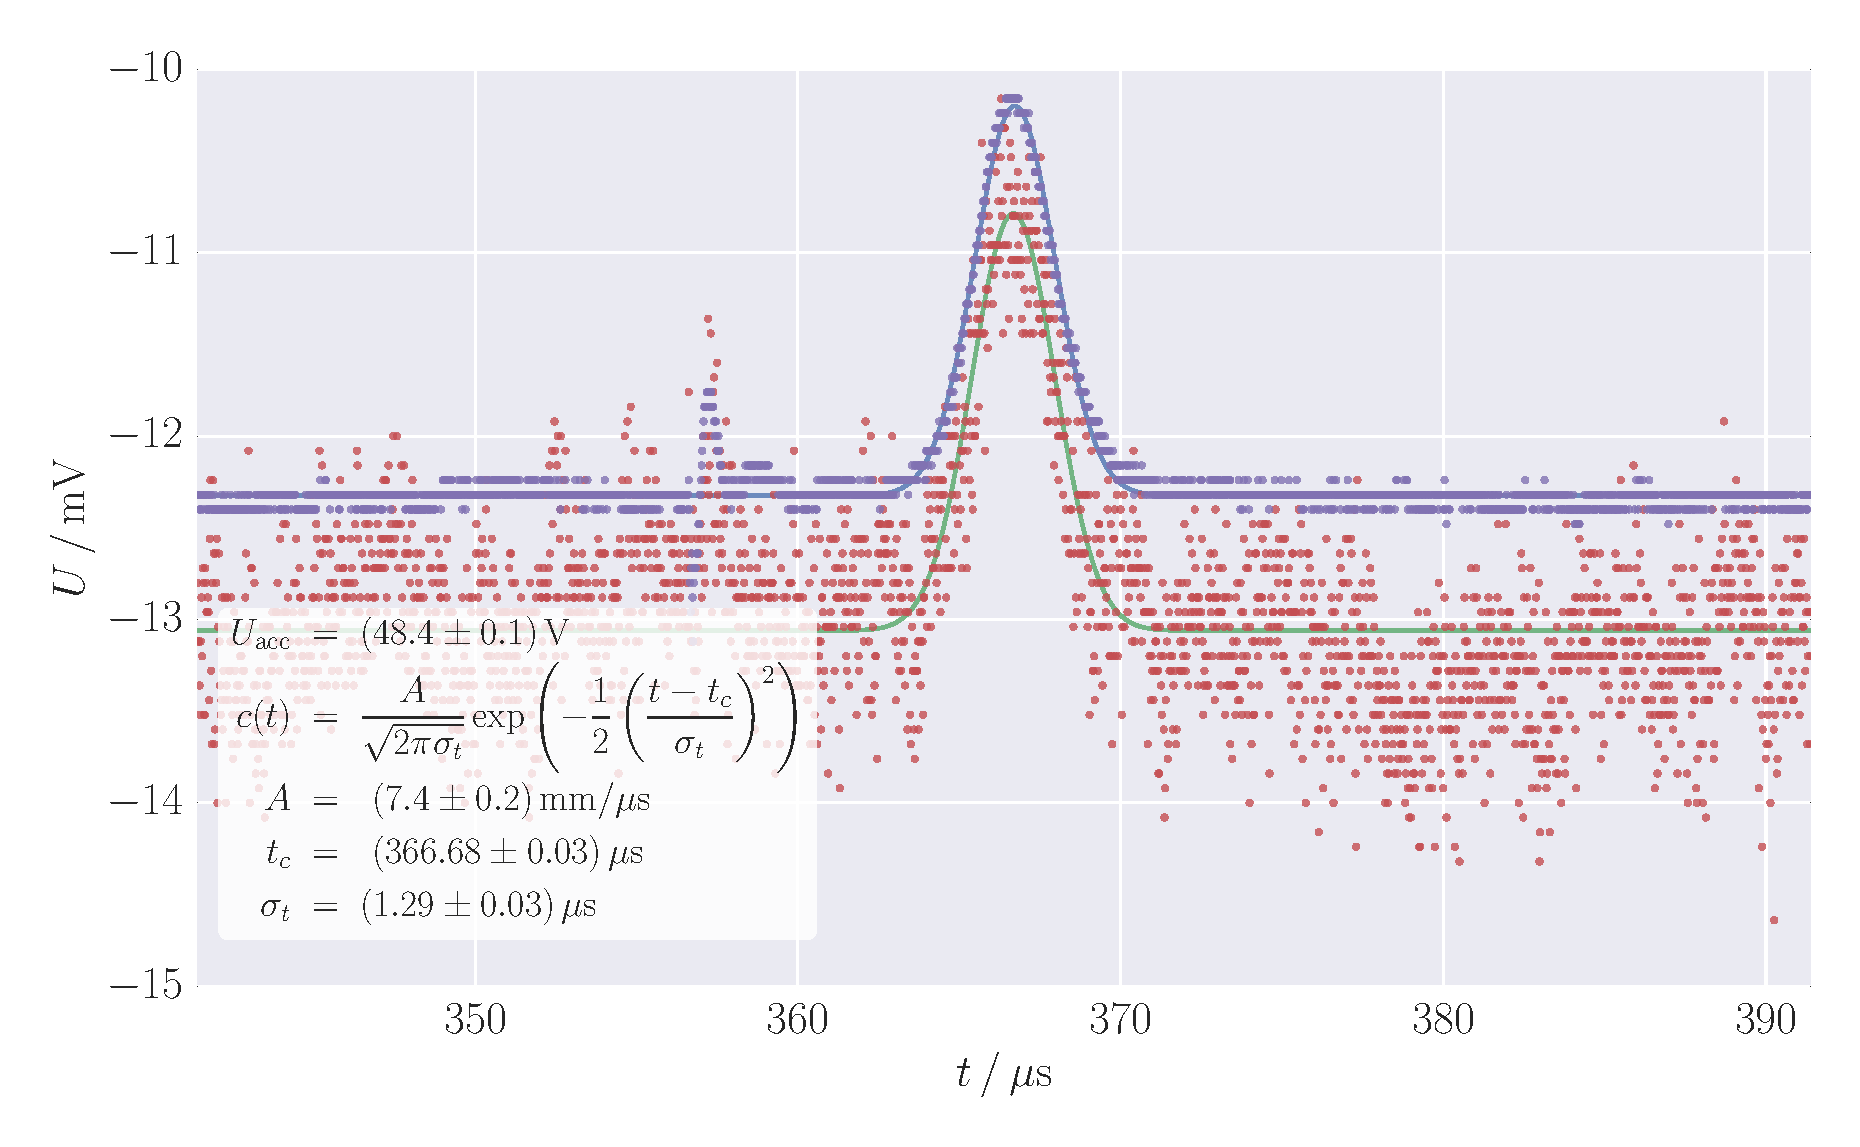
\includegraphics[width=1.0\linewidth]{figures/haynes_shockley_raw_U_39}
        \caption{}
        \label{fig:h_s_raw_U_39}
    \end{subfigure}
    \begin{subfigure}[b]{\pltw}
        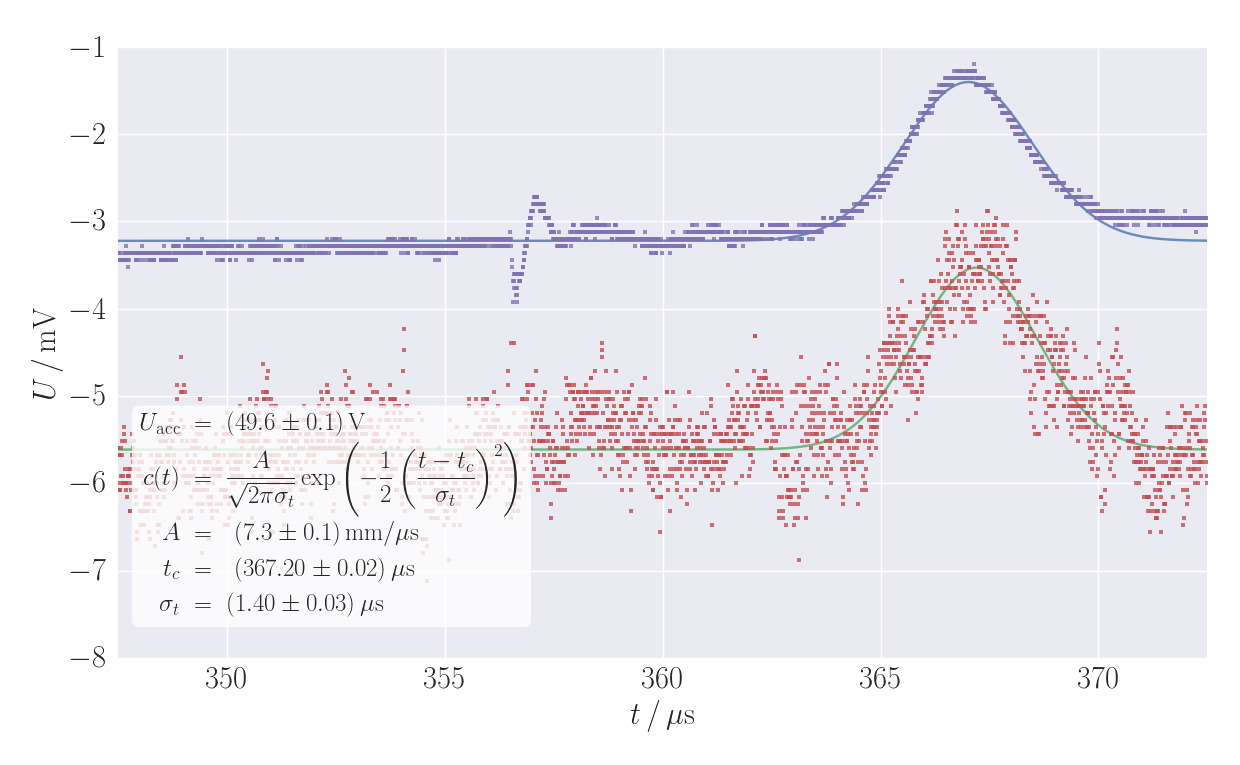
\includegraphics[width=1.0\linewidth]{figures/haynes_shockley_raw_U_65}
        \caption{}
        \label{fig:h_s_raw_U_65}
    \end{subfigure}
    \caption{
        (Continued)
        Haynes \& Shockley experiment, measurement with constant $d$:
        Plots of raw data, averaged data and fitted gaussians. 
        The parameters of the gaussians are displayed in the boxes 
        ($c$ omitted).
        }
    \label{fig:h_s_raw_plots_U_39_65}
\end{figure}

\subsection{Appendix: Handwritten records of the experiment}
%    \includegraphics[width=\linewidth]{appendix/}
    \label{sec:records_band_gap}
\clearpage

